% !TeX encoding = UTF-8

%===============================================================================
% Font options are:
%   plain (default), serif (uses Palladio), sans-serif (uses Paratype Sans)
% Layout options are:
%   article (default, no chapters), book (for longer texts, offers \chapter)
% Paragraph options are:
%   noparskip (default, no spacing between paragraphs), parskip (spaced)
\documentclass[serif,article]{agse-thesis}
\renewcommand{\baselinestretch}{1.5}

% Global parameters, replace with actual values.
\newcommand{\thesisTitle}{Traumapädagogik - wann und wozu und wann nicht mehr?}
\newcommand{\thesisSubtitle}{Zur Attraktivität des \textit{Traumas} für die Pädagogik}
% -> You may use \par (but not \\) to format the title. If you do so, you'll
%    need to manually set the 'pdftitle' attribute below.
\newcommand{\studentName}{Olga Urbaniak}
%===============================================================================

\hypersetup{pdftitle={\thesisTitle}}
\hypersetup{pdfauthor={\studentName}}

\usepackage[font={small,it}]{caption}
\usepackage{enumitem}
\setlist{itemsep=0pt,parsep=0pt,partopsep=5pt,topsep=-\parskip}

\begin{document}

\coverpage[
    student/id=1234567,
    student/mail=olga.urbaniak@fu-berlin.de,
    thesis/type=Bachelorarbeit,            % optional, default: Bachelorarbeit
    thesis/group={Arbeitsgruppe Software Engineering},
                                           % optional, default: AGSE
    thesis/firstAdvisor={1. Gutachterin: Prof. Dr. Ulrike Urban-Stahl},            thesis/secondAdvisor={2. Gutachterin: Prof. Dr. Katrin Kaufmann},           % optional
    thesis/examiner={Prof. Dr. Mia Maus},
    thesis/examiner/2={Prof. Dr. Bob Bär}, % optional
    thesis/date=\today,                    % optional, default: \today
   %title/size=\LARGE,      % set this value to overwrite automatic font size
   %abstract/separate       % toggle this to move the abstract to its own page
]


\renewcommand{\headrulewidth}{0pt}
\clearpage
% !TeX encoding = UTF-8
\pagestyle{fancy}
\fancyhf{} %alle Kopf- und Fußzeilenfelder bereinigen


\clearpage
\tableofcontents

\clearpage
\listoffigures

\clearpage
\renewcommand{\headrulewidth}{0.1pt}
\mainmatter
\setcounter{secnumdepth}{0}
% !TeX encoding = UTF-8
\section{Einführung}

Traumapädagogik bezeichnet eine junge Bewegung, die mit lebensgeschichtlich belasteten Kindern und Jugendlichen arbeitende Fachkräfte unterstützt (vgl. Weiß u. a., 2016: 11). Sie ist als Antwort auf die Überforderung der pädagogischen Praxis mit traumatisierten Kindern und Jugendlichen entstanden (vgl. Kühn 2014: 25). In den letzten Jahren entwickelte sich Traumapädagogik von vereinzelten Konzepten hin zu einer institutionalisierten Form mit eigenen Gremien, Zertifizierungen und Standards (vgl. Schimmer 2016: 439 ff.). Entstanden in der stationären Jugendhilfe, öffnet sich Traumapädagogik für andere pädagogische Arbeitsfelder, etwa Primarerziehung, Bildung und Behindertenhilfe als Bereiche, für die psychotraumatologisches Wissen bedeutsam ist (vgl. Bausum u. a. 2013: 8).

Trauma ist ein aus der Medizin stammender Begriff, der erst in den 1960er-Jahren seine psychiatrisch-psychologische Bedeutung einer psychischen Verletzung erhalten hat (vgl. Anhorn \& Balzereit 2016: 37). Trauma für sich ist keine Diagnose im Sinne einer psychischen Störung (vgl. ebd.), ebenso kein pädagogischer Begriff (vgl. Zimmermann 2016: 47). Dennoch ist sie zu einem so attraktiven Begriff für die pädagogische Praxis geworden, dass sich aus dieser Verbindung eine „eigenständige Fachrichtung“ (vgl. z. B. Bausum u. a. 2013: 8) entwickelt.

Die vorliegende Arbeit beschäftigt sich mit dem Phänomen der Traumapädagogik und geht der Frage nach, ob die pädagogische Praxis einer Traumapädagogik bedürfe. Wann und wozu und wann nicht mehr? Macht der Zugriff auf \textit{Trauma} die pädagogische Praxis handlungsfähiger?

Um sich den Antworten auf diese Fragen zu nähern, wird zunächst erklärt, was Traumapädagogik ist. Eine eindeutige Definition für diese noch junge und heterogene Bewegung gibt es (noch) nicht. Da \textit{Trauma} semantisch und inhaltlich zur Traumapädagogik gehört, die sich wiederum explizit auf die Psychotraumatologie bezieht, wird im ersten Kapitel der Traumabegriff erklärt. Auf dieser Grundlage werden die Entstehung und Institutionalisierung der „neuen Fachdisziplin“ nachverfolgt. Sind diese Hintergründe geklärt, wird im zweiten Kapitel der Blick frei, um sich mit der in der Traumapädagogik geforderten Haltung, den Inhalten der Konzepte sowie mit Traumapädagogik als institutionellem Konzept auseinanderzusetzen. Der Frage, warum es einer Traumapädagogik bedürfe, widmet sich das dritte Kapitel. Dabei sollen die Argumente für die Traumapädagogik, die in der Literatur zu finden sind, gesammelt werden. Das vierte Kapitel reflektiert kritisch das Vorangegangene und untersucht, wofür die Traumapädagogik benutzt wird. Dabei wird sichtbar, dass Traumapädagogik neue Probleme und Fragen generiert. Anschließend wird der Begriff \textit{Traumapädagogik} kritisch hinterfragt, um noch einmal die Frage nach dem Nutzen des \textit{Traumas} für die pädagogische Praxis anders zu stellen.


\setcounter{secnumdepth}{2}
% !TeX encoding = UTF-8
\section{Begriffliche Annäherung}

Der Begriff \textit{Trauma} entstammt dem Griechischen und bedeutet \textit{Wunde} oder \textit{Verletzung} (vgl. Landolt \& Hensel 2008: 14). Dabei wird nicht unterschieden, ob der Körper oder die Seele betroffen ist (vgl. ebd.). Folgendes Kapitel stellt eine erste Annährung an die Beantwortung der Frage dar, was Traumapädagogik sei. Dazu ist der Begriff \textit{Trauma} zu erklären (1.1), was nicht eindeutig möglich ist. Danach werden die in der Literatur vorfindlichen Definitionen der Traumapädagogik vorgestellt (1.2.). Das Kapitel schließt, indem die Entstehung und Institutionalisierung der Traumapädagogik beschrieben werden (1.3).

\subsection{Trauma}
Trauma ist ein Begriff, der in den letzten Jahren sowohl im Alltagsgebrauch als auch in verschiedenen psychosozialen Handlungsfeldern sehr populär geworden ist. Im allgemeinen Sprachgebrauch wird unter Traumatisierung meist eine seelische Verletzung verstanden (vgl. Hantke \& Görges 2012: 53). Der Begriff wird selbst in der Traumaforschung nicht eindeutig benutzt. Nicht immer wird deutlich, ob Trauma das Ereignis, die Auswirkungen, die Symptome oder das Leiden bedeutet (vgl. ebd). Die International Classification of Diseases (Internationale statistische Klassifikation der Krankheiten und verwandter Gesundheitsprobleme, kurz ICD, momentan gültige Fassung: ICD-10) definiert Trauma indirekt als ein „Ereignis oder eine Situation kürzerer oder längerer Dauer, mit außergewöhnlicher Bedrohung oder katastrophenartigem Ausmaß, die bei fast jedem eine tiefe Verzweiflung hervorrufen würde“ (ICD-10-GM 2016, F43.1). Im Diagnostic and Statistical Manual of Mental Disorders (zu Deutsch: Diagnostischer und statistischer Leitfaden psychischer Störungen, Fassung DSM-IV-TR) werden zwei Aspekte genannt, die gleichzeitig erfüllt werden müssen, um von Trauma zu sprechen: (1) das Erleben oder Beobachten eines Ereignisses, das eine ernsthafte Bedrohung der körperlichen oder psychischen Integrität der eigenen oder anderer Personen darstellt; (2) die Reaktionen der betroffenen Person sind von intensiver Furcht, Hilflosigkeit, Grauen und durch aufgelöstes oder agitiertes Verhalten begleitet (vgl. Saß u. a. 2003: 512). Im aktuellsten DSM V entfällt das zweite Kriterium, das sich auf das subjektive Erleben bezieht (vgl. Falkai u. a. 2015: 1111). Mit der Entstehung, der Erfassung, dem Verlauf und der Behandlung der Folgen lebensbedrohlicher und/oder extrem belastender Ereignisse befasst sich Psychotraumatologie (vgl. Landolt \& Hensel 2008: 14), die mit ihrer stressbezogenen Sichtweise (vgl. Hensel 2014: 27) von einem kausalen Zusammenhang zwischen dem Entstehen einer psychischen Störung und belastenden Lebensereignissen ausgeht. Laut Hausmann (2006: 16) beschäftigt sich Psychotraumatologie mit traumatischen Ereignissen und ihren Auswirkungen auf das Erleben und Verhalten von Einzelpersonen und sozialen Systemen. Ein psychisches Trauma sei dabei als ein zumeist plötzlich auftretendes Ereignis zu verstehen, das auf den Betroffenen sehr bedrohlich wirke und zugleich als nicht zu bewältigen erscheine (vgl. Hausmann 2006: 31). Ein Trauma löst intensive Gefühle des Ausgeliefertseins, der Hilflosigkeit, des Entsetzens, der Angst, Verzweiflung oder Wut aus oder führt zu einem Zustand der emotionalen Betäubung und Apathie. Ein psychisches Trauma kann langfristige psychische Symptome verursachen. Die traumatisierende Wirkung eines Ereignisses hängt von der Art des Geschehens sowie von dessen Umständen ab, aber auch von der betroffenen Person, ihren Handlungs- und Bewältigungsmöglichkeiten sowie verschiedenen Schutz- und Risikofaktoren (vgl. ebd.). Die Schutzfaktoren, die unter die Resilienz subsumiert werden und die die Auswirkungen der traumatischen Situationen abschwächen würden, verlieren laut Hensel an Bedeutung, je intensiver und häufiger die Belastung ist (vgl. Hensel 2014: 27). Die klassischen Diagnosen der Anpassungsstörung sowie die posttraumatische Belastungsstörung (PTBS) sind nicht die einzigen und häufigsten Folgen einer Traumatisierung (vgl. ebd.), obwohl hauptsächlich diese zur Verfügung stehen. Zu den typischen PTBS-Symptomen gehören, die traumatischen Erlebnisse in Form von Bildern, Gedanken, Wahrnehmungen oder Halluzinationen (sog. \textit{Flashbacks}) wiederholt zu erleben; mit dem Trauma verbundene Reize zu vermeiden; übertriebene Wachsamkeit. Fehlen diese Symptome, ist dies jedoch keine Garantie dafür, dass kein Trauma vorliegen kann (vgl. Becker 2006: 175). Zu traumatischen Erfahrungen zählen nach klassischem Verständnis hauptsächlich lebensbedrohliche Ereignisse, sexueller Missbrauch oder Misshandlung (vgl. Hensel 2014: 27). Zu chronischen psychischen Fehlanpassungen tragen unter anderem auch solche extremen Belastungen wie der Verlust einer wichtigen Bezugsperson (nicht nur durch Tod) sowie immer wieder im Alltag erlebte Kränkungen (wie Ausgrenzung, psychische Misshandlung und Mobbing) bei (vgl. ebd.). Potenziell traumatisierende Ereignisse sind von unterschiedlicher Art und Dauer. Die amerikanische Kinderpsychiaterin Leonore Teer (1991 zit. nach Landolt \& Hensel 2008: 14) unterscheidet zwei Arten von Traumata:

\begin{itemize}
\item Typ I - einmalige, zeitlich begrenzte, zufällige Traumata (z. B. Naturkatastrophen, Verkehrsunfälle oder Brandkatastrophen), sogenannte Monotraumata
\item Typ II - länger andauernde und wiederholte, teilweise vorhersehbare Geschehnisse (z. B. Sexueller Missbrauch, familiäre Gewalt, Aufenthalt im Kriegsgebiet), sprich: multiple Traumata
\end{itemize}

Des Weiteren können traumatisierende Ereignisse anhand ihrer Ursache klassifiziert und in von Menschen verursachte Ereignisse („man made“) oder durch Naturkatastrophen hervorgerufene und akzidentelle Traumata (z. B. ein Autounfall) eingeteilt werden (vgl. Landolt \& Hensel 2008: 15, siehe Abbildung 1). Dabei geht es immer um ein Ereignis, das eine Bedrohung für das Leben und die körperliche Unversehrtheit des Menschen darstellt (vgl. ebd.). Die neurobiologischen Befunde lassen davon ausgehen, dass traumatische Ereignisse auf der Ebene des Gehirns eine gestörte Informationswahrnehmung bedeuten können (vgl. Landolt \& Hensel 2008: 16).

\begin{figure}[h]
  \centering
  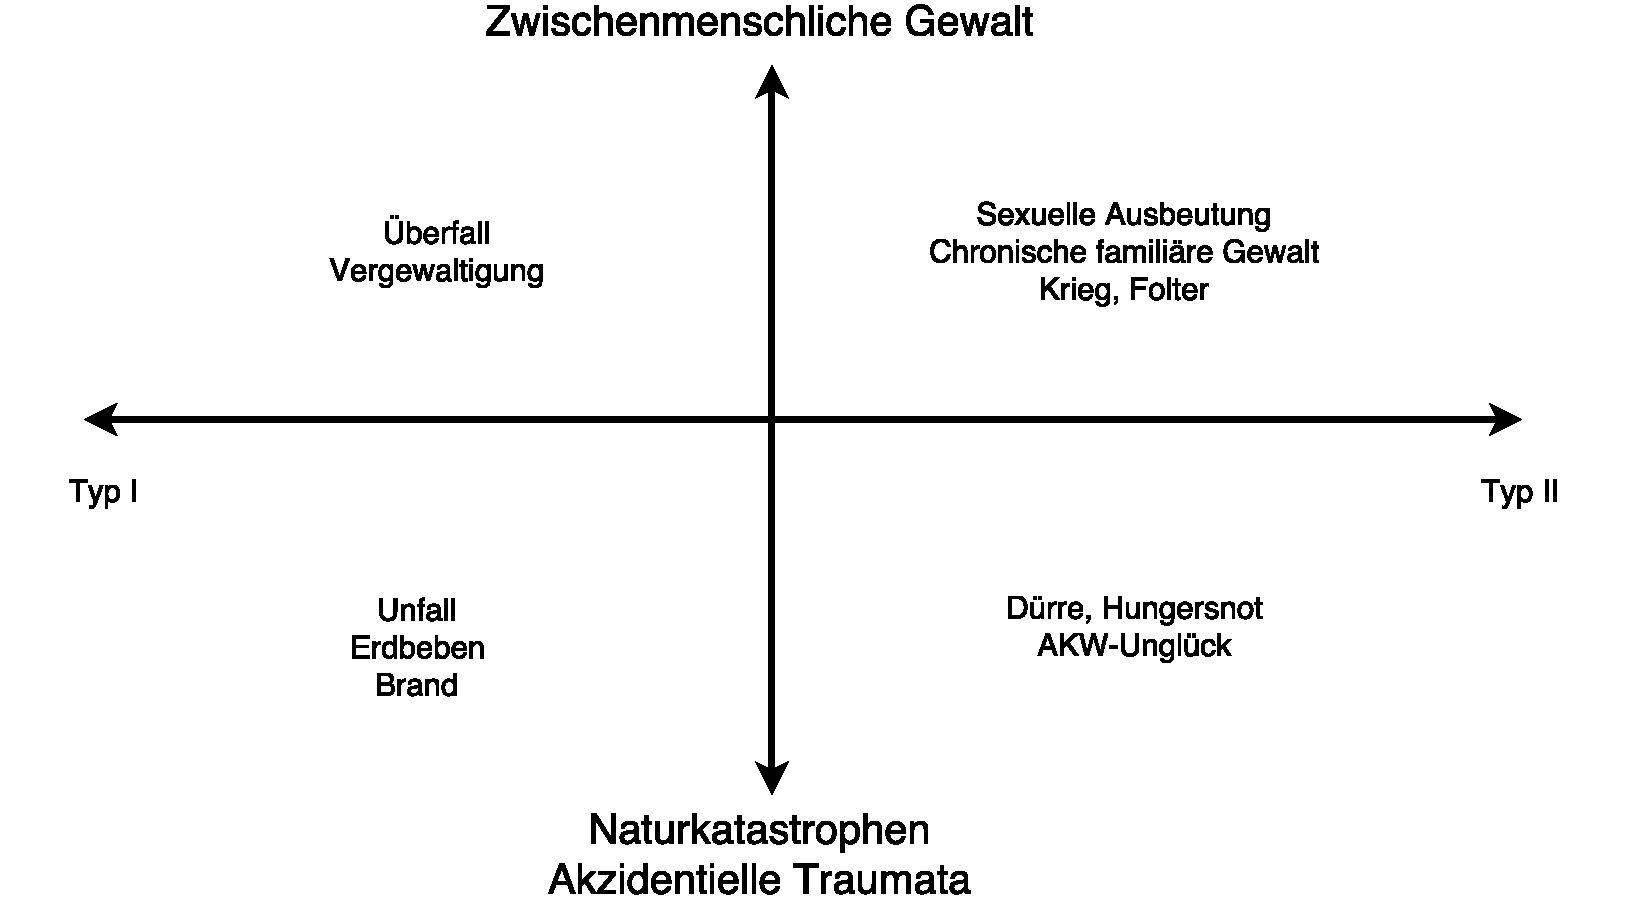
\includegraphics[scale=0.5]{abbildung1}
  \caption
      [Klassifikation traumatischer Ereignisse]
      {Klassifikation traumatischer Ereignisse (nach Landolt, 2004 zit. nach Landolt \& Hensel 2008: 14)}
\end{figure}

Die Entwicklung einer posttraumatischen Reaktion ist als Folge realer Erfahrungen und nicht als Eigenart des Individuums zu verstehen (vgl. Hensel 2014: 28).

\begin{quote}
\small{„Es sind die konkreten Lebensbedingungen, die psychische Symptome verursachen; es sind unbewältigte Lebenserfahrungen im Sinne einer Traumageschichte, die psychisch krank machen. Nur Störungen zu sehen, ohne den Hintergrund der Entstehung zu erkennen und anzuerkennen, bedeutet die Person zu pathologisieren.“ (Huber 2003: 31)}
\end{quote}

Diese Sichtweise ist keineswegs neu. Sie knüpft an die Anfänge der Psychotherapie (Psychoanalyse) und der freudschen Erkenntnis des Zusammenhangs zwischen der Erfahrung des sexuellen Missbrauchs in der frühen Kindheit und den Symptomen (Hysterie) im Erwachsenenalter an (vgl. Hensel 2014: 29 f.). Nach Freud ist ein Trauma „ein Erlebnis, welches dem Seelenleben innerhalb kurzer Zeit einen so starken Reizzuwachs bringt, dass die Erledigung oder Aufarbeitung derselben in normal-gewohnter Weise missglückt, woraus dauernde Störungen im Energiebetrieb resultieren müssen“ (Freud 1961: 284). 

\subsection{Traumapädagogik - Begriff und Definition}
Traumapädagogik wird als „Sammlungsbegriff für [...] Konzepte [benutzt], um die Handlungsfähigkeit der professionellen Fachkräfte wieder herzustellen und traumatisierten Kindern, Jugendlichen und Erwachsenen eine adäquate Teilhabe am sozialen Leben zu ermöglichen“ (Website Traumapädagogik o. J., vgl. Bausum u. a. 2013: 8). Aus den psychotraumatologischen Erkenntnissen sind, so Bausum, abgeleitete Konzeptionen entstanden, die in ihrer Komplexität als eigenständige „Fachrichtung der Traumapädagogik“ zu verstehen seien (ebd.).  

Der Begriff \textit{Traumapädagogik} bleibt schwammig und wird zum Teil unterschiedlich benutzt (vgl. Schmid u. a. 2007: 333). Der Begriff selbst ist vermutlich auf Volker Vogt und Martin Kühn zurückzuführen, die 2002 ein Webprojekt (www.traumapädagogik.de) als ein Diskussionsforum zur kindlichen Traumatisierung in der Pädagogik initiierten (vgl. Kühn 2006: 4; Weiß 2016b: 22). Kühn (2006: 5) distanzierte sich mit der Zeit von der anfangs als Arbeitstitel gedachten Bezeichnung seines Projektes. Der Name \textit{Traumapädagogik} zeige nicht deutlich genug, wozu und mit welchem Ziel gewirkt werden solle. Im Falle seines Konzeptes entscheidet er sich dafür, von einer \textit{Pädagogik} des sicheren Ortes zu sprechen (vgl. Kühn 2006: 4 f.). Kühn definiert Traumapädagogik als Ansatz zur Stabilisierung und Förderung traumatisierter Kinder und Jugendlicher. Sie sei eine notwendige Voraussetzung, Begleitung und Ergänzung eines entsprechenden Therapieprozesses. Daraus ergibt sich die Notwendigkeit eines engen interdisziplinären Austauschs und Diskurses zwischen Pädagogik, Psychotherapie und Psychiatrie (vgl. Kühn 2013: 27). Schmid versteht Traumapädagogik als „die konsequente Anwendung des aktuellen Kenntnisstands der Psychotraumatologie auf das pädagogische Verständnis der betreuten Menschen“ (Schmid 2013: 46). Damit meint er vor allem traumapädagogische Konzepte in der stationären Jugendhilfe als Beispiel für „die konsequente Umsetzung eines innovativen pädagogischen Konzepts, das auf klare psychopathologische Symptome abzielt“ (Schmid 2013: 57). Gemäß seinem Verständnis ist Traumapädagogik eine symptomspezifische, pädagogische Förderung psychisch belasteter Kinder und Jugendlicher (vgl. Schmid 2013: 57). Schmid u. a. (2007: 333) bemängeln, dass der Begriff häufig rein theoretisch besetzt werde, ohne daraus praktische Handlungskonsequenzen oder pädagogische Konzepte abzuleiten. Die Traumapädagogik entstand hauptsächlich an der Schnittstelle zwischen Kinder- und Jugendpsychiatrie/-psychotherapie und Jugendhilfe, die geholfen hat, „aus der Psychotraumatologie heraus milieutherapeutische Konzepte abzuleiten oder althergebrachte Konzepte der Heimerziehung aus einer psychotraumatologischen und neurobiologischen Perspektive heraus zu begründen“, so Schmid u. a. (2014: 174). Weiß (2016b: 29) sieht die Möglichkeit, die Haltungen und Methoden der Traumapädagogik vielseitig anzuwenden. Eine traumapädagogische Haltung sei eine solche, die für jede Pädagogik gültig sein sollte. Denn extremer Stress und traumatische Erfahrungen seien im Leben vieler Menschen verbreitet (vgl. ebd.). Weiß betont den Unterschied zwischen einerseits der Traumabearbeitung als der Bewältigung durch die Betroffenen und andererseits der Traumaarbeit, die die Begleitung durch psychosoziale Fachkräfte sei (vgl. Weiß 2016b: 20 f.). Sie versteht Traumapädagogik als notwendige Unterstützung traumatisierter Kinder und Jugendlicher im pädagogischen Alltag als Teil der Traumaarbeit (vgl. ebd.). Weiß u. a. definieren Traumapädagogik als eine junge Fachrichtung, die es sich zur Aufgabe gemacht hat, Fachkräfte, die mit traumatisch belasteten Kindern und Jugendlichen im Arbeitsalltag konfrontiert sind, zu unterstützen (vgl. Weiß u. a. 2016: 11). Dies soll durch spezifische Fort- und Weiterbildungen und die Schaffung tragfähiger Strukturen in den Institutionen geschehen (vgl. ebd.). Die Traumapädagogik sei als Antwort auf die Fragen der Praxis nach dem Umgang mit traumatisch belasteten Kindern und Jugendlichen in pädagogischen Arbeitsfeldern entstanden und fokussiere in der Auseinandersetzung mit dieser Frage drei Bereiche (vgl. Bausum u. a. 2013: 8):

\begin{itemize}
\item Begegnung zwischen Kind und pädagogischer Fachkraft 
\item Handlungssicherheit der pädagogischen Fachkraft 
\item Institutionelle Strukturen der Einrichtung
\end{itemize}

Die vorhandenen Definitionen der Traumapädagogik zeigen, dass diese noch ganz in den Anfängen steckt und anscheinend um ihre Berechtigung und Anwendungsbereiche kämpft. Die Traumapädagogik, trotz direkter Bezüge zur Psychotraumatologie, sagt nicht immer eindeutig aus, was unter Traumatisierung verstanden wird, was es wiederum erschwert, den Gegenstand und die Handlungsfelder zu bestimmen.

\subsection{Entstehung und Institutionalisierung der Traumapädagogik}
Die Anfänge der heute unter dem Begriff Traumapädagogik subsumierten Konzepte sind in stationären und teilstationären Einrichtungen der Kinder- und Jugendhilfe ab Mitte der 1990er-Jahre zu suchen (vgl. Weiß 2016b: 20). Ihnen vorausgegangen sind Ende der 1980er-Jahre Prozesse der Enttabuisierung des Themas sexueller Gewalt in der Kinder- und Jugendhilfe und folglich die Erweiterung des Blickwinkels auf andere Formen der Gewalt gegen Kinder. Stationäre Jugendhilfe, Pflegeeltern und Behindertenhilfe sind Bereiche, die Bedarf an entsprechenden Konzepten außerhalb des psychotherapeutischen Rahmens melden (vgl. Weiß 2016b: 20 f.).

Der Prozess der Professionalisierung und Institutionalisierung der Traumapädagogik beginnt zu Anfang dieses Jahrhunderts mit ersten Publikationen, Fort- und Weiterbildungen bis hin zur Gründung einer Bundesarbeitsgemeinschaft Traumapädagogik (BAG-TP), die sich zum Ziel setzt, das psychotraumatologische Wissen in verschiedene pädagogische Arbeitsfelder in Form von Diskussionen und Fortbildungen in traumabezogener Pädagogik zu tragen. Ihre Ziele sieht die BAG-TP in „Entwicklung, Förderung und Forschung von/zu Konzeptionen und Projekten in Erziehungs-, Bildungseinrichtungen und der Jugend-/Behindertenhilfe. Themen sind dabei u. a. die psychischen, physischen, sozialen und gesellschaftspolitischen Grundlagen und Folgen von Stressreaktionen bei Kindern und Jugendlichen auf traumatische Lebensereignisse und entsprechenden pädagogischen Begegnungen und Interventionsmöglichkeiten“ (BAG-TP 2011: 2). BAG-TP formuliert 2011 Traumapädagogische Standards in der stationären Kinder- und Jugendhilfe sowie, zusammen mit der Deutschsprachigen Gesellschaft für Psychotraumatologie (DeGPT), Kriterien für ein Curriculum Traumapädagogik/Traumazentrierte Fachberatung. Nach einer entsprechenden Weiterbildung, die momentan an 36 Instituten in Deutschland angeboten wird (vgl. DeGPT/Fachverband Traumapädagogik o. J.), kann eine Qualifikation für Traumapädagogik/Traumazentrierte Fachberatung erworben werden.

Hantke (2012: 198) beschreibt den Prozess der Entstehung der Traumapädagogik und ihrer Institutionalisierung vor dem Hintergrund der Ausdifferenzierung und Entgrenzung der therapeutischen, beraterischen und pädagogischen Bereiche. Die neuen Überlegungen, die aus der Traumatheorie resultieren, wurden in erste therapeutische Verfahren umgesetzt und diese dem Bereich der psychologischen Psychotherapie zugeschrieben. Damit sei der Zugang zu dem neuen Wissen und den Verfahren für viele psychosoziale Fachkräfte begrenzt gewesen. Die neuen, traumazentrierten Methoden, Denk- und Erklärungsansätze sollen Einzug in die stationäre Versorgung und in ambulante Settings in Form neu entstehender Traumapädagogik- und Traumaberatungscurricula gefunden haben (vgl. ebd.).

% !TeX encoding = UTF-8
\section{Traumap{\"a}dagogik - Haltung, Konzepte, traumasensible Organisationsentwicklung}

Traumapädagogik charakterisiert sich durch eine Grundhaltung, die als Basis des pädagogi-schen Handelns zu verstehen ist und sich in einem wertschätzenden pädagogischen Verständ-nis des Kindes zeigt (vgl. Schmied \& Lang 2012: 339). Aus den verschiedenen pädagogischen Konzepten, die zunächst aus der Praxis heraus entstanden sind, lassen sich handlungsleitende Inhalte herausarbeiten (vgl. Rothdeutsch-Granzer u. a. 2015: 178 f.). Traumapädagogik als konsequente Anwendung des psychotraumatologischen Wissens in der Ausgestaltung des pädagogischen Alltags und ein wertschätzendes Verständnis der betreuten Menschen berück-sichtigt alle Ebenen einer Organisation (vgl. Schmid \& Lang 2012: 339 ff.; BAG-TP 2011: 5) und kann als ein traumasensibler Organisationsentwicklungsprozess verstanden werden. Im Folgenden werden die traumapädagogische Haltung (2.1), wichtigste traumapädagische Kon-zepte und deren Inhalte (2.2) sowie die Traumap{\"a}dagogik als ein pädagogischs Konzept (3.3) fokussiert.

\subsection{Traumapädagogische Haltung}

Eine traumasensible Grundhaltung stellt die Basis für die Entwicklung traumapädagogischer Konzepte sowie eine Orientierung für das praktische und pädagogische Handeln dar (vgl. BAG-TP 2011: 4). Dabei soll das Wissen um die möglichen Folgen belastender Erlebnisse berücksichtigt werden, und es sollen die Ressourcen der Kinder und Jugendlichen im Mittel-punkt stehen (vgl. ebd.). Für die Entstehung der Traumap{\"a}dagogik seien Psychotraumatologie ebenso wie Soziale Arbeit, bindungstheoretische Grundlagen und Resilienzforschung, Neurobiologie und die therapeutischen Wissenschaften von Bedeutung (vgl. Weiß 2016b: 22). Traumap{\"a}dagogik beziehe sich auf Reformpädagogik, emanzipatorische Pädagogik und ver-trete das in der humanistischen Pädagogik und Psychologie begründete Menschenbild (vgl. Weiß 2016b: 23). Auf dieser Basis ist eine Reihe von Konzepten entstanden, die sich zwar in Inhalten und Gewichtung im pädagogischen Handeln unterscheiden, allerdings eine gemein-same Grundhaltung haben (vgl. ebd.). Die traumapädagogischen Standards formulieren dazu folgende fünf Handlungsansätze (vgl. BAG-TP 2011: 5 ff.):

\begin{itemize}
\item „Die Annahme des guten Grundes – Alles was ein Mensch zeigt, macht Sinn in seiner Geschichte!“ (ebd.: 5) 
\item „Wertsch{\"a}tzung – Es ist gut so, wie du bist!“ (ebd.: 5) 
\item „Partizipation – Ich traue dir was zu und {\"u}berfordere dich nicht!“ (ebd.: 6) 
\item „Transparenz – Jeder hat jederzeit ein Recht auf Klarheit!“ (ebd.: 6) 
\item „Spaß und Freude – Viel Freude tr{\"a}gt viel Belastung“ (ebd.: 7)
\end{itemize}

Im Zentrum der traumapädagogischen Haltung steht die Annahme des guten Grundes (vgl. Weiß 2016b: 23; Rothdeutsch-Granzer u. a. 2015: 177). Das Verhalten des Kindes wird dabei im Kontext seiner Biografie und Entwicklung als normale Reaktion auf eine außerordentliche Belastung verstanden. Das Kind soll in seinem Wesen und samt seinen Schwierigkeiten, die als Überlebensstrategien zu verstehen sind, angenommen und wertgeschätzt werden (vgl. ebd.). Transparenz im pädagogischen Alltag und die Teilhabe an der Gestaltung der eigenen Lebensbedingungen ermöglichen Kindern und Jugendlichen, Autonomie, Kompetenz und Zugeh{\"o}rigkeit zu erleben (vgl. BAG-TP 2011: 6). Dies sind wichtige Faktoren, die die seelische Gesundheit beeinflussen und eine Alternative zu den vorangegangenen Erfahrungen wie Gewalt, Vernachl{\"a}ssigung und/oder Missbrauch anbieten. Spaß und Freude zu erleben, wirkt ausgleichend zu den belastenden Erlebnissen, die die Gefühlswelt in ein Ungleichgewicht bringen (vgl. ebd.). Die traumapädagogische Haltung solle nicht nur den Kindern und Jugendlichen gegenüber gelten, sondern die MitarbeiterInnen und KooperationspartnerInnen miteinschließen (vgl. Schmid \& Lang 2012: 345).

\subsection{Traumapädagogische Konzepte – handlungsleitende Inhalte}
Traumapädagogik als Sammlung von Konzepten, die traumatisierte Mädchen und Jungen sowie junge Erwachsene im pädagogischen Alltag unterstützen, ist aus der pädagogischen Praxis entstanden. Diese Konzepte weisen einige Gemeinsamkeiten auf, vor allem in Bezug auf die Grundhaltung (siehe 2.1), als auch Unterschiede in Inhalten und im Handeln (vgl. Weiß 2016b: 23). Aus diesen Konzepten lassen sich handlungsleitende Inhalte für das pädagogische Handeln herausarbeiten (vgl. Rothdeutsch-Granzer u. a., 2015: 178 f.; siehe Abbildung \ref{fig:inhalte})

\begin{figure}[h]
  \centering
  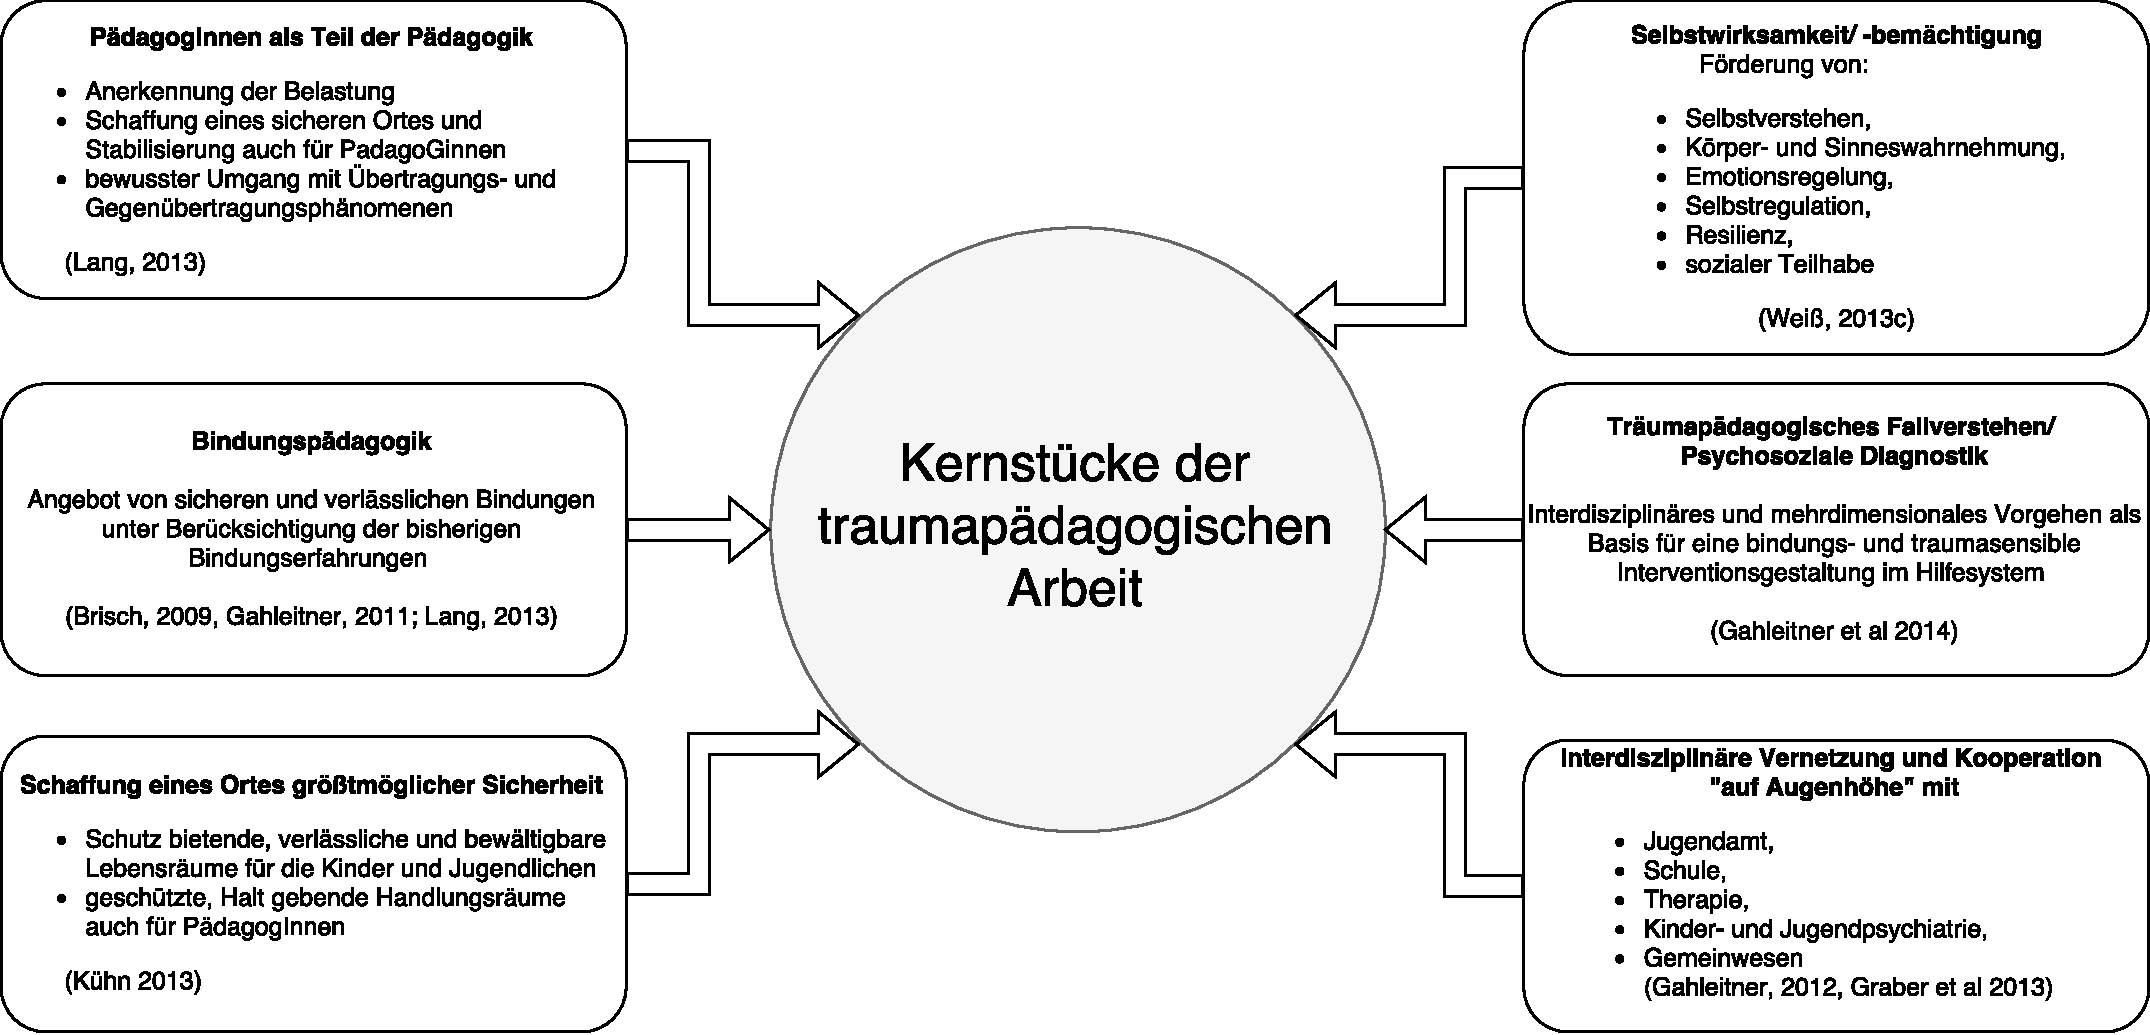
\includegraphics[scale=0.45]{abbildung2}
  \caption
      [Handlungsleitende Inhalte der traumapädagogischen Arbeit]
      {Handlungsleitende Inhalte der traumapädagogischen Arbeit (nach Rothdeutsch-Granzer u. a., 2015: 179)}
  \label{fig:inhalte}
\end{figure}

Kühn (2014: 21) bezeichnet drei Kernkonzepte als richtungsweisend in der Traumap{\"a}dagogik: \textit{Pädagogik des sicheren Ortes} (vgl. Kühn 2006), \textit{Traumazentrierte Pädagogik} nach Uttendörfer (2008) und \textit{Pädagogik der Selbstbemächtigung} nach Weiß (2016a). Mittlerweile sind weitere Konzepte und Anwendungen entstanden, die die Vielfältigkeit der Handlungsfelder zeigen, in denen psychotraumatologisches Wissen gefragt ist. Das sind, um einige Beispiele zu nennen: \textit{Traumapädagogische Gruppenarbeit} nach Bausum (2013), \textit{Stabilisierung und (Selbst-)Fürsorge für PädagogInnen} (Lang 2013), \textit{Traumapädagogik in der Schule} (Ding 2013, Zimmerman 2016) und \textit{Milieutherapeutische Konzepte} (Gahleitner 2011). Auch in weiteren Handlungsfeldern und für AdressatInnen wie z. B. Ehe- und Familienberatung, Gefangenenseelsorge, Gewaltprävention, Frauenhäuser, Wohneinrichtungen für unbegleitete minderjährige Flüchtlinge etc. sei traumapädagogisches Wissen gefragt (vgl. Hantke 2015: 118).  

Die gemeinsamen Inhalte der Konzepte sind in Bezug auf den \textit{sicheren Ort} und die Bedeutung der Bindung sowie positiver Beziehungserfahrungen für die Traumabearbeitung am weitesten entwickelt (vgl. Weiß 2016b: 27). Viele Konzepte adaptieren (psycho-)therapeutische Methoden, um z. B. mit Fertigkeitstrainings oder Notfallkoffern die Emotionsregulation zu begleiten (vgl. ebd.: 28). Einige Konzepte betonen die Wichtigkeit und Bedeutung der traumatischen Übertragungs- und Gegenübertragungsreaktionen (vgl. Kessler 2016: 123 ff.; Schmid 2013: 48) und formulieren entsprechende Interventionen. Die Traumabearbeitung als ein Prozess der Selbstbemächtigung nach Weiß (2016b: 20) beinhaltet unter anderem: traumabedingte Einstellungen und Überzeugungen zu verändern; das Geschehen in die eigene Lebensgeschichte einzuordnen; die Möglichkeit, in der Gegenwart Sinn zu finden; Körperfürsorge und Körpergewahrsein zu entwickeln; Selbstregulation zu erlernen; die traumatischen Erinnerungen und den traumatischen Stress zu kontrollieren sowie soziale Teilhabe zu ermöglichen. Dieses Konzept betont vor allem die Expertenschaft der Kinder und Jugendlichen. Ihnen soll das Wissen über Traumatisierung zur Verfügung gestellt werden (vgl. ebd.).  

Schmid und Lang (2012: 347) sehen Psychoedukation als bedeutenden Bestandteil der Traumap{\"a}dagogik. Ziel sei es, den Kindern und Jugendlichen ihre Reaktionen und Symptome, neurobiologische Abl{\"a}ufe, das Entstehen von Spannungszust{\"a}nden, K{\"o}rperreaktionen und Dissoziationen\footnote{Das Einstellen der Aussenwahrnehmung und ein tranceartiger Zustand, begleitet von einem Verlust des Körpers und Zeitgefühls, der räumlichen Orientierung, der Schmerzwahrnehmung, oft mit einem Derealisationserleben verbunden (vgl. Schmid u. a. 2010; 49 f.). Gefühle und Gedanken werden getrennt und im Falle der Traumatisierung kann ein Verlust der Integration der Erinnerungen an die Vergangenheit eintreten (vgl. Weiß u. a. 2016; 460).} etc. in einer altersangemmessenen und verständlichen Form mit bildhafter Sprache und grafischer Unterstützung zu erklären. Dabei sei die Botschaft wichtig, dass Symptome und Schwierigkeiten der Heranwachsenden eine normale, menschliche Reaktion auf v{\"o}llig unnormale und unmenschlichet Erlebnisse darstellen. Wichtig sei es, dass das Kind und die mit ihm arbeitenden Erwachsenen die gleiche Terminologie benutzten, um eine gemeinsame Sprache für spätere Interventionen und Analyse von schwierigen Situationen zu entwickeln (vgl. Schmid \& Lang 2012: 347).

\subsection{Traumapädagogik als Konzept}
Die BAG-TP sieht die Notwendigkeit, die Erkenntnisse der Psychotraumatologie und der Hirnforschung in den Institutionen, in denen traumatisierte Mädchen und Jungen betreut werden, umzusetzen (vgl. BAG-TP 2011: 4 f.). Klare Haltungen, F{\"o}rderans{\"a}tze und Methoden, die in der Umsetzung traumap{\"a}dagogischer Konzepte unerl{\"a}sslich seien, bilden die Grundlage f{\"u}r die von der BAG-TP formulierten Standards zur traumap{\"a}dagogischen Arbeit in Einrichtungen der station{\"a}ren Kinder- und Jugendhilfe. Im Mittelpunkt eines traumapädagogischen Konzepts steht laut der BAG-TP, verlässliche Beziehungen im Alltag aufzubauen und zu gewährleisten, die Traumatisierten sozial und emotional zu stabilisieren sowie das Selbstvertrauen der zu betreuenden Kindern und Jugendlichen aufzubauen und zu stärken (vgl. ebd.). Dabei soll die traumapädagogische Grundhaltung (siehe 2.1) als Voraussetzung institutionell durchg{\"a}ngig erkennbar bleiben (vgl. BAG-TP 2011: 5 ff.). Eine Einrichtung, die traumapädagogisch arbeitet, soll zu einem sicheren Ort werden, an dem betroffene Kinder und Jugendliche „neue, erg{\"a}nzende Erfahrungen machen k{\"o}nnen, sich selbst und ihre Handlungsstrategien verstehen lernen, Entwicklungshemmnisse aufholen und sichere Bindungserfahrungen machen k{\"o}nnen“ (BAG-TP 2011: 4). Die Entwicklung dieses Ortes soll alle Beteiligten mit einbeziehen und als ein institutioneller und kontinuierlicher Prozess verstanden werden. Die Einführung eines traumapädagogischen Konzepts im Sinne eines sicheren Ortes soll mehrere Ebenen einer Institution miteinschließen (vgl. ebd.). Schmid (2013: 49) versteht das Einbeziehen der MitarbeiterInnen und der strukturellen Abläufe in die (trauma-)pädagogische Konzeption als zentral. Um den Kindern und Jugendlichen einen stabilisierenden, sicheren Rahmen zu bieten, bedarf es solcher MitarbeiterInnen und Strukturen, die selbst stabil und selbstwirksam sind. Die MitarbeiterInnen und Teams brauchen, um bei den Krisen stabilisierend zu wirken, dieselben Fertigkeiten wie die Kinder und Jugendlichen selbst (vgl. ebd.). Schmid (2013: 49) beschreibt eine Institution, die ein traumapädagogisches Konzept umsetzt, als eine Versorgungskette, am Anfang derer das Kind steht, das im Alltag unterstützt werden soll (siehe Abbildung \ref{fig:konzept}). Hierzu bedarf es jedoch stabiler und stabilisierender Strukturen auf allen Ebenen der Organisation (vgl. ebd.).

\begin{figure}[h]
  \centering
  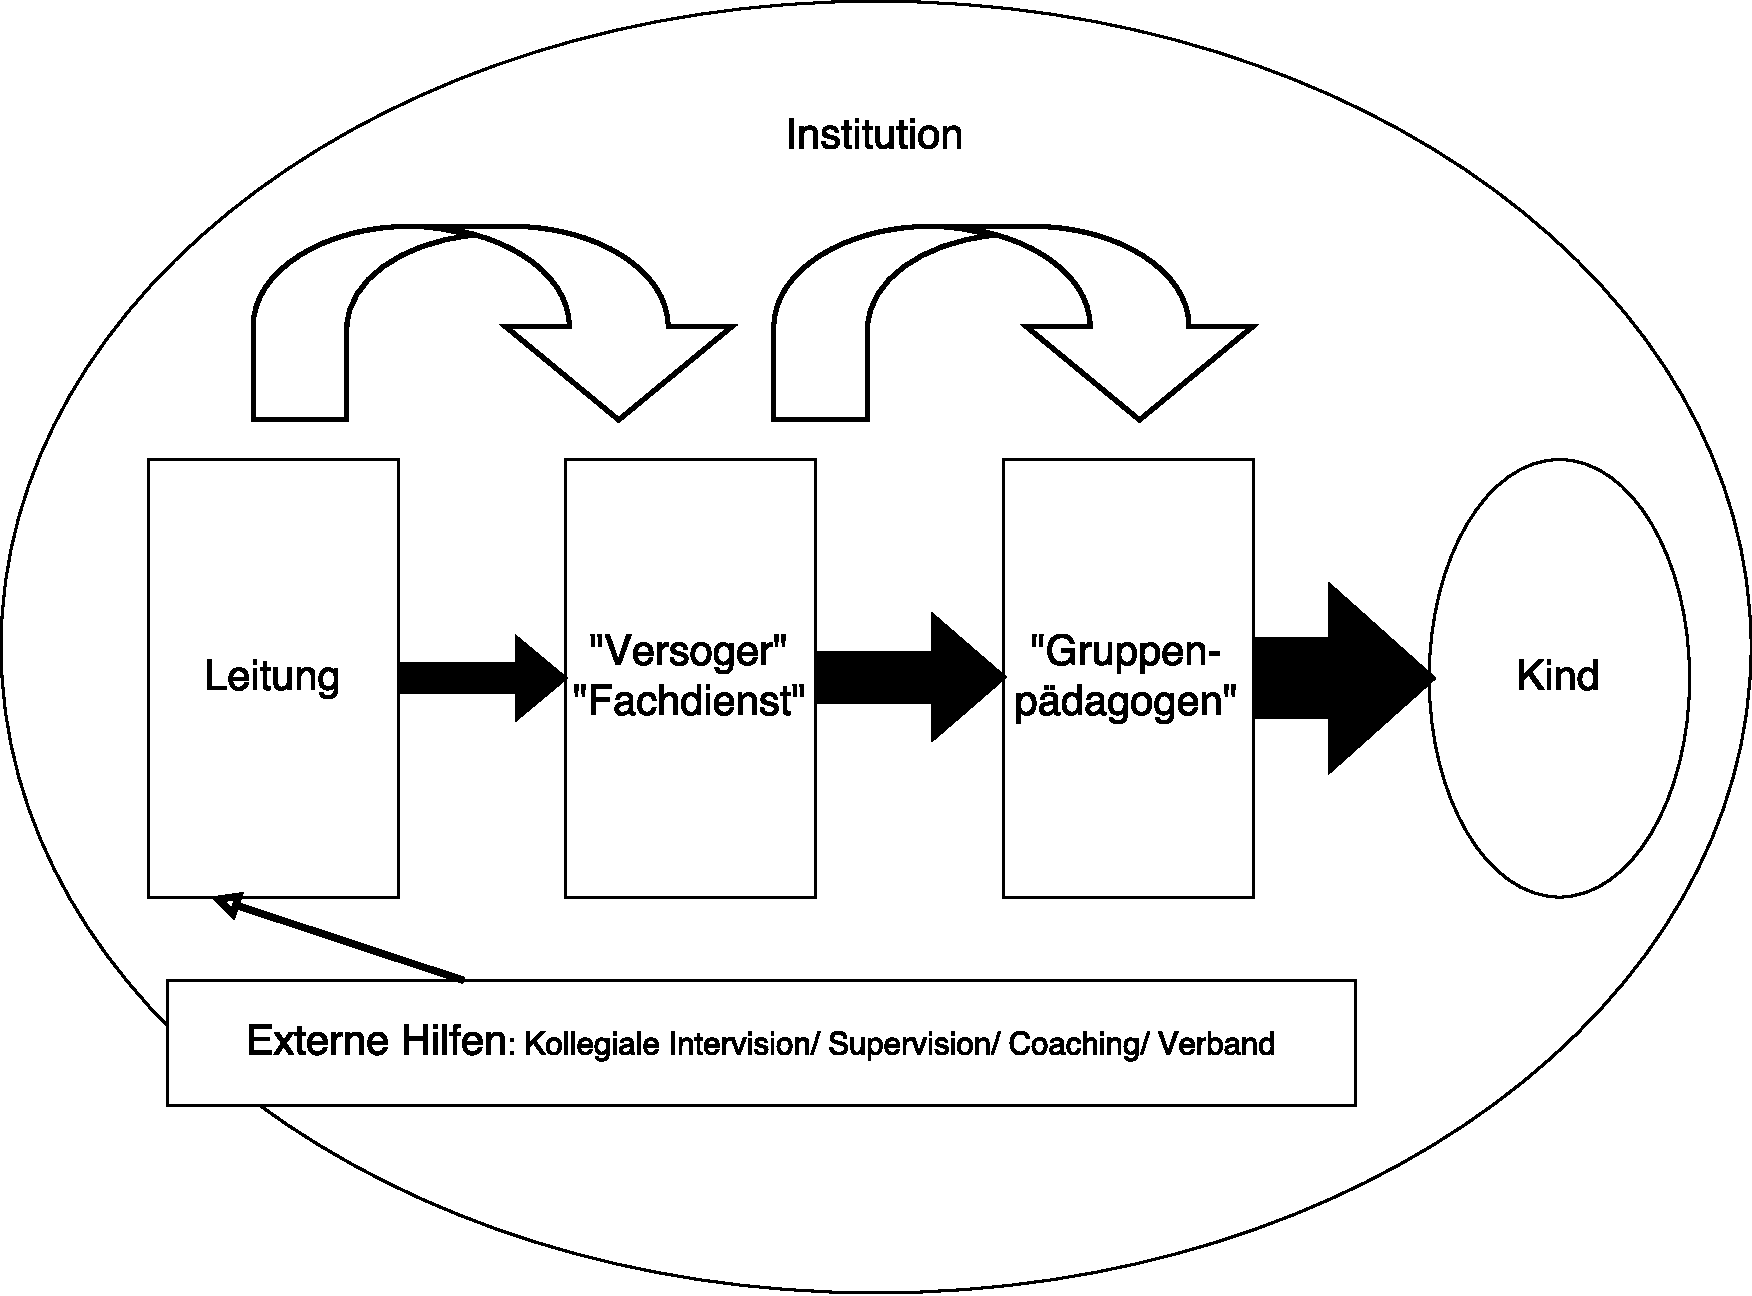
\includegraphics[scale=0.3]{abbildung3}
  \caption
      [Konzept einer Versorgungskette]
      {Konzept einer Versorgungskette (nach Schmid 2013: 49)}
  \label{fig:konzept}
\end{figure}

Traumap{\"a}dagogik sowie traumapädagogische Standards können laut Schirmer (2016: 443 f.) als Paradigmenwechsel in der Heimerziehung gewertet werden. Dieser besteht darin, dass die pädagogischen Fachkräfte, Kinder und Jugendlichen und die institutionellen Strukturen in das pädagogische Konzept im Sinne einer wertgeleiteten Organisations- und Personalentwicklung mit der zugrunde liegenden wertschätzenden verstehender Grundhaltung einbezogen werden. Diese Haltung richtet sich darauf, das „unerwünschte“ Verhalten reflexiv zu verstehen und gemeinsam nach Lösungen und pädagogisch nachvollziehbaren pädagogischen Interventionen zu suchen (vgl. ebd.).

% !TeX encoding = UTF-8
\section{Gute Gründe für Traumap{\"a}dagogik – worüber gesprochen wird}

Traumapädagogik ist als Antwort auf die Überforderung der pädagogischen Praxis mit traumatisierten Kindern und Jugendlichen entstanden (vgl. Kühn 2014: 25). Dieser Überforderung will Traumapädagogik mit entsprechenden Haltungen und Konzepten begegnen. Vorliegendes Kapitel widmet sich der Frage, warum es der Traumapädagogik bedürfe. Im Folgenden werden Argumente, die in der Literatur zu finden sind und für die Traumapädagogik sprechen sollen, beschrieben. Das Kapitel fokussiert: die Häufigkeit der Belastungen der Kinder und Jugendlichen (3.1), deren besondere Bedarfe (3.2), den Beitrag der Traumapädagogik zur Entlastung der pädagogischen Praxis (3.3) sowie ihre Bedeutung für den pädagogischen Alltag (3.4).

\subsection{Es sind viele!}
Die hohen Zahlen der Kinder und Jugendlichen, die belastenden, traumatischen Erlebnissen ausgesetzten waren, soll die Bedeutung der Psychotraumatologie für deren (therapeutische) Unterstützung beweisen (vgl. Landolt \& Hensel 2008: 13). Daten, die die tatsächliche Anzahl traumatisierter Kinder und Jugendlicher in Deutschland verlässlich abbilden könnten, gibt es nicht (vgl. Bundesministerium für Familie, Senioren, Frauen und Jugend [BMFSFJ] 2009: 238). Häufig werden Studien und Zahlen zitiert, die die Anwesenheit psychisch belasteter Kindern und Jugendlicher in verschiedenen pädagogischen Institutionen beweisen sollen. Die berichteten Zahlen der potenziell oder tatsächlich Traumatisierten variieren zwischen 60 und 85\% bei den fremdplatzierten Kindern (vgl. Schmid 2013: 36 ff.). Als besonders belastet gelten laut diesen Ergebnissen Mädchen und Jungen, die in den stationären Einrichtungen der Jugendhilfe untergebracht sind und besonders häufig Vernachlässigung und Misshandlungsrisiken ausgesetzt waren (vgl. ebd.). Der Großteil der Kinder in Heimen weise Typ-II-Traumatisierungen auf und leide an einer komplexen posttraumatischen Belastungsstörung oder Traumaentwicklungsstörung (s. u., vgl. Schmid 2013: 37). Viele Kinder und Jugendlichen in der Jugendhilfe zeigten in der Diagnostik gleichzeitig mehrere psychische Erkrankungen, was deren besonderen Unterstützungsbedarf beweise (vgl. Schmid 2013: 38). Somit gelte für die Einrichtungen der station{\"a}ren Jugendhilfe, dass früh misshandelte, missbrauchte und vernachlässigte Kinder eher die Regel als Ausnahme seien (vgl. ebd.: 36). Aus diesen Erkenntnissen sowie aus der Tatsache, dass die KlientInnen der Jugendhilfe auch externe Einrichtungen wie z. B. Schulen besuchen, werden Bedarfe an den traumapädagogischen Konzepten auch für diese abgeleitet (vgl. Möhrlein \& Hoffart 2014: 91ff.). Momentan ist ein Anstieg wissenschaftlicher Publikationen zum Thema der Lebenssituationen minderj{\"a}hriger Fl{\"u}chtlinge zu beobachten (vgl. Reinelt u. a. 2016: 232 f.). Das Interesse an der Thematik der psychischen Gesundheit gefl{\"u}chteter Kinder und Jugendlichen steigt. Besonders viel wird über das m{\"o}gliche Auftreten einer posttraumatischen Belastungsst{\"o}rung und ihre Behandlung publiziert (vgl. ebd.).

\subsection{Besondere Bedarfe traumatisierter Kinder und Jugendlicher}
Der spezifische pädagogische Bedarf der komplex traumatisierten Kinder und Jugendlichen ergibt sich laut Schmid (2013: 47) aus den Traumafolgen. Einmalige traumatische Ereignisse sind meist leichter zu erkennen und therapeutisch zu begleiten, als das bei den chronischen und wiederkehrenden Erfahrungen (z. B. Kindesmisshandlung) der Fall ist.  

Die systematische Auseinandersetzung mit kindlichen Reaktionen auf traumatische Ereignisse ist in der Kinderpsychotherapie noch recht jung (vgl. Landolt \& Hensel 2008: 13). Erst im Jahre 1988 wurde das Vorhandensein der posttraumatischen Belastungsstörung (PTBS) auch bei Kindern anerkannt (vgl. ebd.). Gleichzeitig ist die PTBS weder die typische noch die häufigste Traumafolgestörung bei Kindern und Jugendlichen (vgl. Hensel 2014: 27). Traumatische Erlebnisse in der Kindheit wirken sich auf die emotionale, kognitive und soziale Entwicklung der Kinder und Jugendlichen aus (vgl. Purtscher-Penz 2015: 95). Folgen einer lebensbedrohlichen Erfahrung, etwa eines Unfalls, sexuellen Missbrauchs, Verlusts einer nahen Bezugsperson etc., können psychische Erkrankungen, somatische Beschwerden, Lernprobleme sowie Störungen des Sozialverhaltens sein. Auch stressbezogene Alltagserfahrungen können zu traumareaktiven Folgeerkrankungen führen. Wiederholte Stressereignisse und chronisches Stresserleben verursachen eine komplexe Traumatisierung bei Kindern und Jugendlichen. Nur wenige dieser Kinder zeigen traumaspezifische Folgeerkrankungen im klinischen Sinne (vgl. ebd.). Da die vielfältigen und komplexen Folgen der frühkindlichen Traumatisierung in den bisherigen Diagnosen nicht berücksichtigt seien, wird eine Diagnose von entwicklungsbezogenen Traumafolgestörungen (vgl. Purtscher-Penz 2015: 97) bzw. Traumaentwicklungsstörungen (mehr dazu: Schmid u.a. 2010) diskutiert. Die Herausforderungen für die (sozial-)pädagogische Praxis, die sich laut Schmid (2013: 43) aus den Folgen komplexer Traumatisierungen ergeben, fasst die untenstehende Abbildung \ref{fig:folgen} zusammen.

\begin{figure}[h]
  \centering
  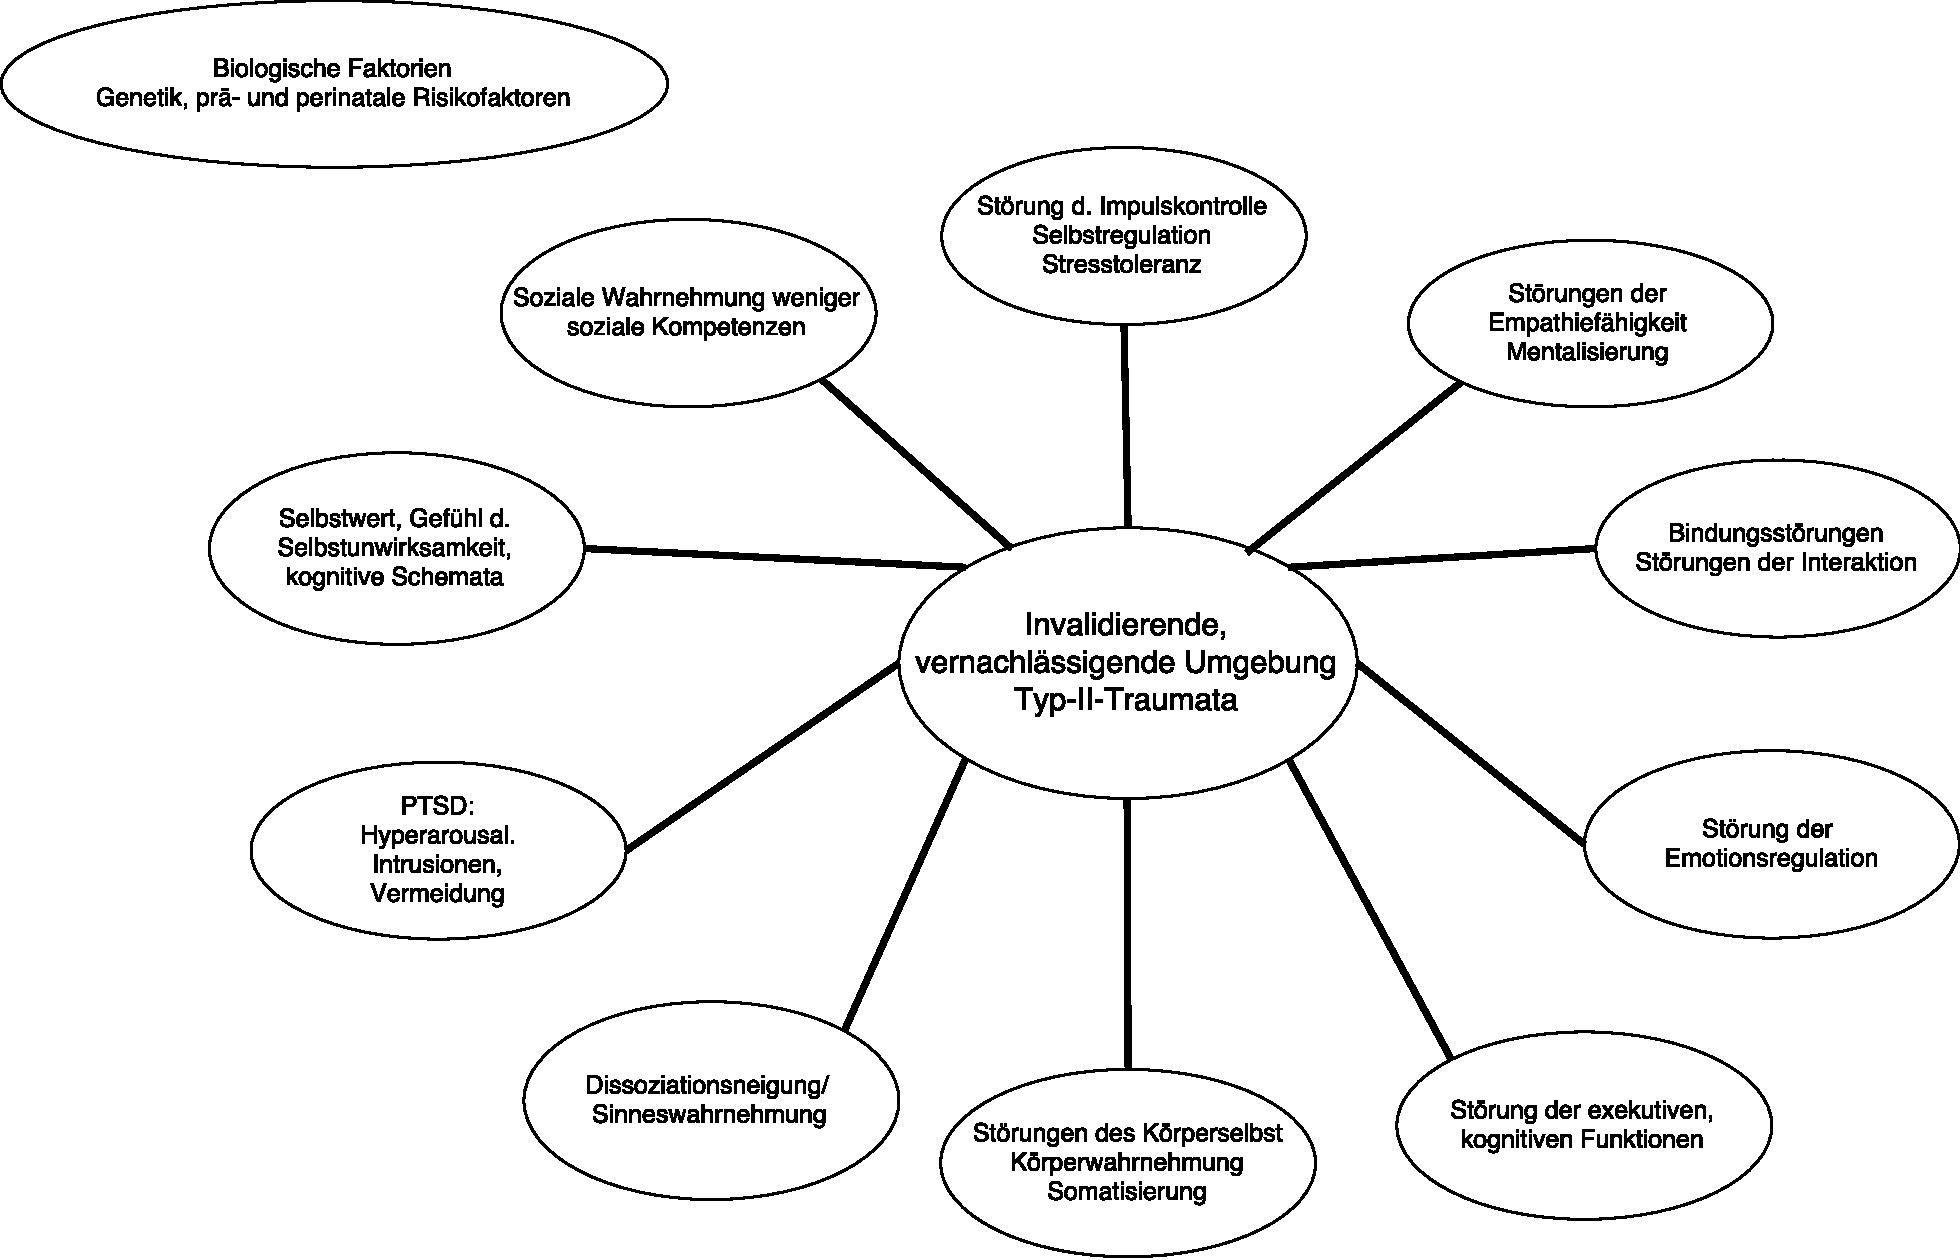
\includegraphics[scale=0.45]{abbildung4}
  \caption
      [Folgen komplexer Traumatisierungen für die Pädagogik]
      {Folgen komplexer Traumatisierungen für die Pädagogik (nach: Schmid 2013: 43)}
  \label{fig:folgen}
\end{figure}

Diese Herausforderungen lassen wiederum auf einen spezifischen pädagogischen Bedarf der betroffenen Kinder und Jugendlichen sowie entsprechende Interventionen schließen (vgl. Schmid 2013: 47; vgl. Abbildung \ref{fig:ansatzpunkte}: \pageref{fig:ansatzpunkte}). Da diese Kinder häufige Beziehungsabbrüche und Wechsel von Bezugspersonen erlebt haben, brauchen sie Sicherheit und Verlässlichkeit im Alltag, was die Verlässlichkeit von Bezugspersonen, getroffenen Vereinbarungen und Absprachen bedeutet (vgl. Purtscher-Penz 2015: 99). Belastende Lebenserfahrungen zu bewältigen, ist ein lebenslanger Prozess. Bei Kindern und Jugendlichen kann es auf kognitiven, emotionalen und sozialen Entwicklungsstufen zur Neubearbeitung der vergangenen Erfahrungen kommen. Dies ist keineswegs als Rückfall oder „Scheitern“ der vorangegangenen Therapie zu verstehen (vgl. ebd.).

\subsection{Entlastung der Praxis – Wiederherstellung der Handlungsfähigkeit}
Die ersten, am meisten ausgearbeiteten und praxiserprobten traumapädagogischen Konzepte kommen aus der stationären Jugendhilfe. Die PädagogInnen in der Jugendhilfe seien immer wieder mit Kinder und Jugendlichen konfrontiert, die sie an die Grenzen ihrer Handlungsmöglichkeiten brächten (vgl. Kühn 2013: 24). Traumap{\"a}dagogik sei „als Antwort auf die Erfolglosigkeit oder Nichtwirksamkeit bestimmter Konzepte in den letzten Jahren direkt aus der pädagogischen Praxis entstanden“ (Kühn 2013: 25). Die Geschichte der Heimerziehung sei „eine Geschichte von Trauma und Retraumatisierung“ (ebd.), und bis heute werde sich selten gründlich mit dem Scheitern der einzelnen Hilfsmaßnahmen auseinandergesetzt. Meistens werden die zu Betreuenden als nicht tragbar für die Einrichtung erachtet und weiterverwiesen (vgl. ebd.).

Auch Schmid (2013: 38 ff.) thematisiert die häufigen Beziehungsabbrüche den Jugendlichen (auch innerhalb der Jugendhilfe), die sich in stationären Maßnahmen befinden, was sich wiederum auf deren Bindungsfähigkeit auswirke und die aktuellen Beziehungen beeinflusse könne. Die Abbrüche und Wechsel der Institutionen entstehen laut Schmid (vgl. ebd.) oft infolge von Überforderung des sozialpädagogischen Teams mit den Symptomen des Kindes oder Jugendlichen, was zu Gefühlen der Ohnmacht und geringer Selbstwirksamkeit der Fachkräfte führt. Nicht selten wird in diesen Fällen psychotherapeutische Unterstützung für das betroffene Kind gefordert. Weiter beschreibt Schmid, wie die Erwartung an psychotherapeutische Interventionen nicht erfüllt werden kann, wenn zwischen der Pädagogik und der Psychotherapie kein gemeinsames Fallverständnis gelingt. Als nächste Maßnahme für das Kind oder den Jugendlichen (und zur Entlastung des Teams) soll nicht selten die Aufnahme in die Kinder- und Jugendpsychiatrie erfolgen. Die erforderlichen intensiven Betreuungssettings sind allerdings nicht ausreichend vorhanden, und viele Kinder und Jugendliche, die ein intensiveres Angebot benötigen, müssen abgewiesen werden. Um diesen „Kreislauf aus Ohnmacht und Ausstoßung“ (Schmid 2013: 42) zu unterbrechen, seien pädagogische Konzepte entwickelt worden, die an den Traumafolgestörungen und deren pädagogischen Folgen ansetzten. Belastete Kinder zeigen Verhaltensweisen, die ohne das Wissen um potenzielle traumabedingte Ursachen nicht adäquat beantwortet werden bzw. die Symptomatik verschärfen können (vgl. ebd.). Die MitarbeiterInnen und Teams müssen, so Schmid (2014: 185), vor Burn-out und der Möglichkeit einer sekundären Traumatisierung, die sich aus dem Arbeitskontext mit Traumatisierten ergeben, geschützt werden. Die traumapädagogischen Konzepte begründen gemäß Schmid die Notwendigkeit, Strukturen zu schaffen, die die Resilienz der MitarbeiterInnen fördern. Denn die Qualitätssicherung dient dem Wohle der PatientInnen (vgl. ebd.).

\subsection{Zur Bedeutung der Traumapädagogik im pädagogischen Alltag}
Der Bedarf an traumazentrierter Pädagogik wird aus den Möglichkeiten, die der pädagogische Alltag zur Unterstützung der Bewältigung der Traumatisierungsfolgen bietet, abgeleitet (vgl. Weiß 2016b: 20; Hantke 2015: 123 f.). Kinder und Jugendliche, die extremen Traumatisierungen ausgesetzt worden sind, zeigen oft Symptome, die ihren Alltag, auch in pädagogischen Kontexten, beeinflussen. Die pädagogischen Konzepte, die Erkenntnisse der Psychotraumatologie berücksichtigen, unterstützen die Fachkräfte, indem ihnen eine Alternative im Verstehen der Verhaltensweisen der Kinder angeboten wird sowie einige methodische Zugänge zur Verfügung gestellt werden, um mit den Symptomen des Traumas wie Übererregung, Dissoziation oder traumatische Übertragung im Alltag zu arbeiten (siehe z. B. Weiß 2016a: 290 ff.). In der Gesellschaft sowie unter den PädagogInnen wird meist die Psychotherapie als geeignete Methode zur Behandlung von Folgen der psychischen Traumata angesehen (vgl. Weiß 2003: 65). Die Auseinandersetzung mit den Traumafolgen und psychischen Störungen im Allgemeinen wird somit an den geschlossenen Raum der Therapie delegiert, so Weiß. An dieser Stelle wird gefordert, therapeutisches Wissen in die P{\"a}dagogik in einem Konzept der Zusammenarbeit von P{\"a}dagogik und Therapie zu integrieren (vgl. Weiß 2013: 20).

Mittlerweile stehen mehrere traumpsychotherapeutische Verfahren zur Verfügung, die zugleich ihre Einschränkungen aufweisen (Übersicht bei Landolt \& Hensel 2008). Unabhängig von der Therapierichtung werden drei Phasen der Traumaverarbeitung unterschieden: (1) Stabilisierung, (2) Traumabearbeitung und (3) Integration (vgl. Landolt \& Hensel 2008: 20; Huber 2003: 19). Als Standard für die psychotherapeutische Behandlung von Traumafolgen gilt, die Betroffenen nicht zu früh mit den traumatischen Erfahrungen zu konfrontieren (vgl. Purtscher-Penz 2015: 98). Zuerst soll eine stabile und tragfähige Beziehung aufgebaut werden. Kinder und Jugendliche brauchen Sicherheit, Geborgenheit und Verlässlichkeit. Erst dann können sie sich mit der traumatischen Erfahrung auseinandersetzen. Diese Auseinandersetzung ist als eine traumaspezifische psychotherapeutische Intervention durchzuführen, so Purtscher-Penz. Ziel der therapeutischen Intervention ist es, die traumabezogene Symptomatik wie Angstsymptome, einschränkendes Vermeidungsverhalten ebenso zu reduzieren wie dissoziative Zustände. In einigen Fällen kommt ergänzende psychopharmakologische Behandlung bei sehr ausgeprägter Angstsymptomatik oder Schlafstörungen hinzu (vgl. ebd.).  

Schmid u. a. (2007: 335) warnen vor unreflektierter und vordergründiger Übernahme prim{\"a}r therapeutischer Techniken in andere Settings. F{\"u}r den Erfolg einer Maßnahme sei p{\"a}dagogische Kernarbeit zur Stabilisierung entscheidender (vgl. ebd.). Komplex traumatisierte Kinder und Jugendliche brauchen neben der Psychotherapie auch eine adäquate Pädagogik im Alltag, die Sicherheit und Kontinuität gewährleistet (vgl. Purtscher-Penz 2015: 99; Hensel 2014: 34). Die aus der Traumatisierung resultierenden Beeinträchtigungen, besonders bei komplex Traumatisierten, wirken im Alltag und bedürfen entsprechender pädagogischer Interventionen, so Schmid (2013: 47, siehe Abbildung 5). Diese können auch im pädagogischen Alltag verfolgt werden. Dazu gehört, einen sicheren Ort zu vermitteln, der vor Retraumatisierungen\footnote{Ein Zustand der Betroffenen Person, in der eine erneute Erinnerung an das traumatische Erlebnis direkt zu einer erh{\"o}hten Symptombelastung f{\"u}hrt (vgl. Maercker 2009; 16).} schützt und das Kind oder den Jugendlichen stabilisiert; „korrigierende Beziehungserfarungen“ durch motivierte und stabile Erwachsene anzubieten und die Emotionsregulation durch das Erlernen spezifischer Fertigkeiten zu verbessern. Die Verbesserung der Selbst-, Fremd- und Körperwahrnehmung kann die Dissoziationsneigung reduzieren. Ressourcenorientierung, Partizipation und Transparenz im Alltag sind aufgrund der vielfachen Erfahrungen des Kontrollverlustes und zur Überwindung der „Selbstunwirksamkeitserwartung [sic]“ wichtig (vgl. Schmid 2013: 47).

\begin{figure}[h]
  \centering
  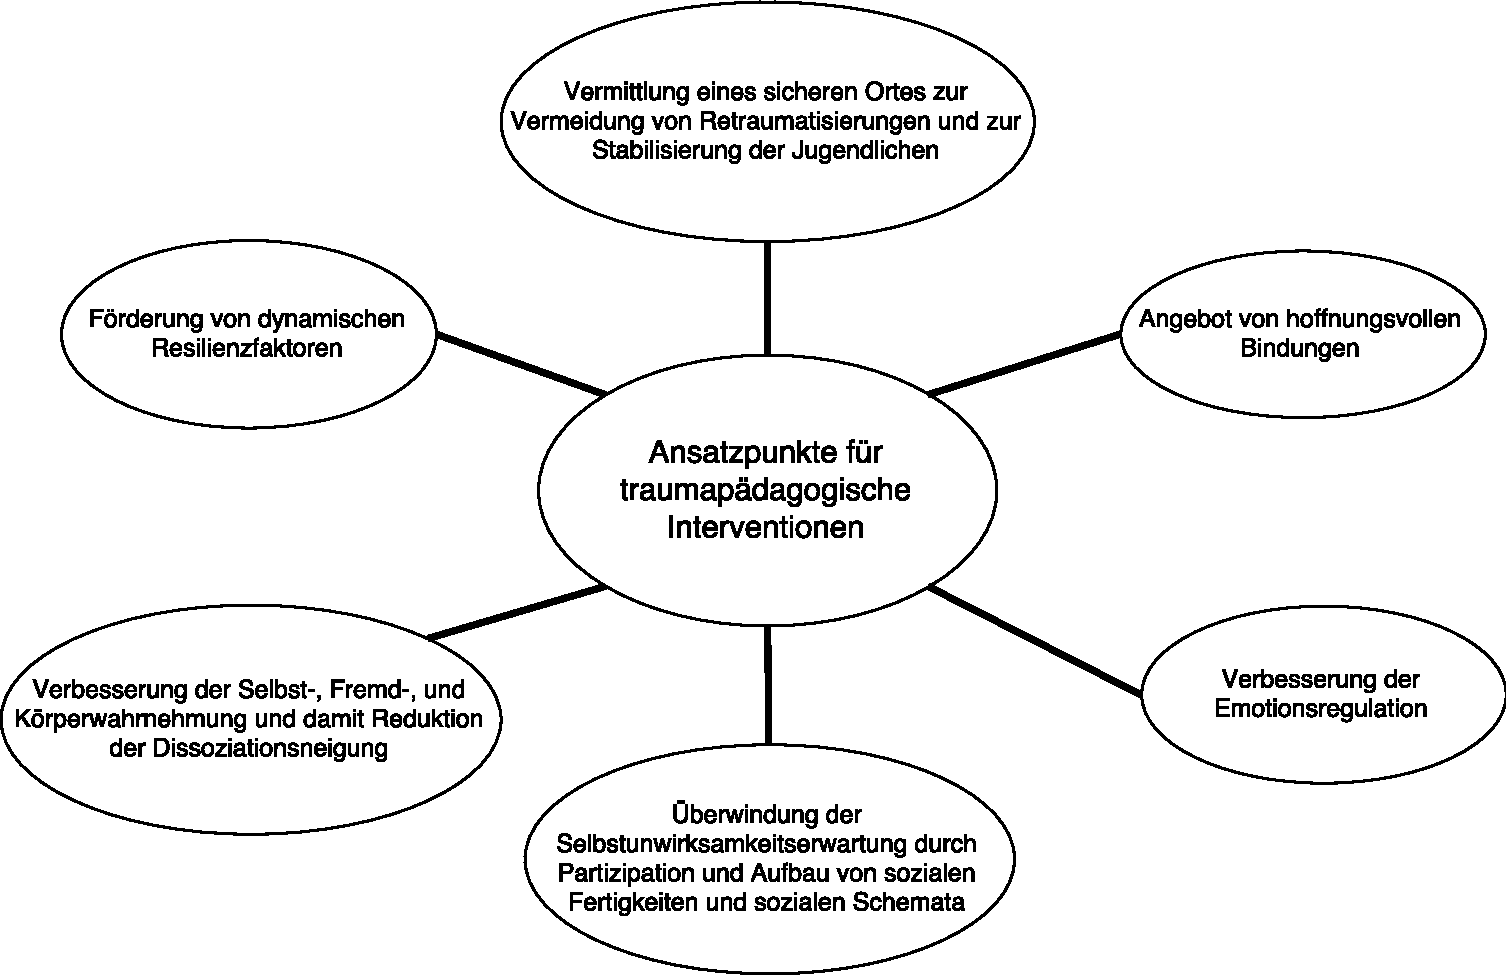
\includegraphics[scale=0.5]{abbildung5}
  \caption
      [Ansatzpunkte für traumapädagogische Interventionen]
      {Ansatzpunkte für traumapädagogische Interventionen (nach Schmid 2008 zit. nach Schmid 2015: 179)}
  \label{fig:ansatzpunkte}
\end{figure}

Weiß (2013: 18 ff.) vertritt den Standpunkt, dass die Verwendung von Erkenntnissen der Traumatheorie und Traumaforschung nicht therapeutischen SpezialistInnen und WissenschaftlerInnen vorbehalten werden sollte. Vielmehr sei es wichtig, diese Erkenntnisse im Interesse der betroffenen M{\"a}dchen und Jungen und der sie begleitenden P{\"a}dagogInnen auf ihre Anwendbarkeit im pädagogischen Kontext zu {\"u}berpr{\"u}fen, da „die Unterst{\"u}tzung traumatisierter M{\"a}dchen und Jungen außerhalb des individualisierten Rahmens von Therapie auch in der P{\"a}dagogik sehr wirksam sein kann“ (Weiß 2013: 21 f.). Die therapeutische Hilfe orientiere sich idealerweise in erster Linie an dem Kind, seinem Wunsch, Alter, seiner Lebensgeschichte, dem aktuellen Wohlbefinden und seiner Stabilität (vgl. Weiß 2013: 180). Ziele der Therapie seien: korrigierende und wiedergutmachende Erfahrungen sowie Unterstützung bei der Entwicklung der Ich-Kräfte. Die Therapieziele seien auch gekoppelt an die Reaktionen der Bezugspersonen und könnten unter Umständen die Kinder und Jugendlichen in erneute Konfliktsituationen bringen (vgl. ebd.: 182). „Eine therapeutische Unterstützung bei der Verarbeitung traumatischer Erfahrungen kann nur hilfreich sein, wenn sie sorgfältig als Teil im gesamten Hilfeprozess eingebettet ist“ (ebd.). Kühn (2014: 21 f.) betont die Überschätzung der therapeutischen Möglichkeiten durch die pädagogischen Fachkräfte, was wiederum zur Unterschätzung und Entwertung der eigenen Fachkompetenz führe (ebd.). Unumstritten bleibt, dass im Rahmen der Traumap{\"a}dagogik keine Traumaexposition (Traumakonfrontation) stattfinden soll. Eine deutliche Abgrenzung zur psychotherapeutischen Intervention sei wichtig (vgl. Schmid u.a. 2007: 335).

Zusammenfassend lassen sich auf der Suche nach der Begründung für die „neue Fachdisziplin“ Traumapädagogik unter anderen vier Argumente identifizieren:

\begin{enumerate}
\item Die Anzahl der durch traumatische Erfahrungen belasteten Kinder und Jugendlichen in den pädagogischen Handlungsfeldern sei hoch.  
\item Diese Kinder und Jugendliche hätten traumabedingt besondere Bedarfe, die besonderer (trauma-)pädagogischer Maßnahmen bedürften.  
\item Die pädagogischen Fachkräfte seien ohne entsprechender Unterstützung und aufgrund der Herausforderungen, die die Traumatisierung mit sich bringe, besonderen Belastungen ausgesetzt und stießen auf Grenzen ihrer Handlungsmöglichkeiten (bis hin zur sekundären Traumatisierung der Fachkräfte).  
\item Dabei biete der pädagogische Alltag viele Möglichkeiten, die betroffene Kinder und Jugendliche in ihrer Traumabearbeitung zu unterstützen. Im Mittelpunkt dieser Überlegungen stünden vorrangig Fachkräfte und Kinder und Jugendliche, die in den stationären und teilstation{\"a}ren Einrichtungen der Jugendhilfe betreut und versorgt würden.
\end{enumerate}

% !TeX encoding = UTF-8
\clearpage
\section{Macht \textit{Trauma} die Praxis handlungsfähiger?}
Die besonderen Bedarfe der traumatisierten Kinder und Jugendlichen und die Überforderung der Fachkräfte sollen die Notwendigkeit der Veränderungen in pädagogischen Institutionen begründen (siehe Kapitel 3). Allerdings wird diesen Bedarfen mit bekannten, pädagogischen und organisatorischen Maßnahmen begegnet. Die kindzentrierten Anteile sind als „sehr konsequente Umsetzung einer guten altbekannten Pädagogik“ (Schmid \& Lang 2012: 343) beschreibbar. Das Neue an der Traumapädagogik besteht darin, die Begründung für die Handlungskonzepte aus der psychotraumatologischen Perspektive herzuleiten (vgl. ebd.). Dabei ist die Verbindung zum Traumabegriff weder eindeutig, noch scheint sie notwendig zu sein. Im Folgenden wird Traumapädagogik auf die Frage hin reflektiert, wem diese einen Nutzen bringe und wozu sie das \textit{Trauma} brauche (4.1). Anschließend wird der Begriff \textit{Traumapädagogik} kritisch hinterfragt (4.2).

\subsection{Gute Gründe für Traumapädagogik? Kritische Gedanken}
Traumapädagogische Leitgedanken bewegen sich im Spannungsfeld zwischen den von den praktisch arbeitenden Fachkräften geforderten Haltungen, ihrem Wissen und ihren anzuwendenden Methoden einerseits und der Adressierung der institutionellen Rahmenbedingungen andererseits, die wiederum nicht losgelöst von den sozialen und politischen existieren. Das Argument, das die Handlungsunfähigkeit der pädagogischen Fachkräfte mit den besonders herausfordernden traumatisierten KlientInnen begründet, kann wirken, als ob die pädagogische Praxis, vor allem in den stationären Jugendhilfe, die schwer belasteten Kinder und Jugendlichen „bräuchte“, um auf ihre sie an sich überfordernden Arbeitsbedingungen aufmerksam zu machen und institutionelle Veränderungen zu legitimieren. Sind das wirklich die traumatisierten, belasteten Kinder und Jugendlichen, die die pädagogische Praxis herausfordern? Die in Kapitel 3 gesammelten Argumente weisen darauf hin, dass betroffene Kinder und Jugendliche traumapädagogische Angebote brauchen. Früh und komplex traumatisierte Menschen, vor allem Kinder und Jugendliche, haben in der Vergangenheit zu wenig Beachtung erfahren (vgl. BMFSFJ 2009: 238). Gesellschaftliche Veränderungen, steigende Anforderungen an Professionalisierung der pädagogisch Handelnden (vgl. Zimmermann 2016: 12 ff.), ausgebauter Kinderschutz, Inklusionsförderung an den Schulen, viele geflüchtete Jungen und Mädchen, die momentan die Jugendhilfe, das Gesundheits-, aber auch das Bildungssystem beschäftigen, überfordern oft die pädagogischen Fachkräfte und Institutionen, die auf Abhilfe hoffen.

Traumapädagogik scheint zunächst eine Lösung anzubieten. Sie trifft momentan auf eine Zeit, die dankend das Angebot annimmt, ohne es zu hinterfragen. Viele Praktiker aus verschiedenen Arbeitsfeldern melden Interesse an psychotraumatologischem Wissen an. Viele Weiterbildungs- und Fortbildungsinstitute sind entstanden, die momentan stark nachgefragt werden (vgl. Schirmer 2016: 439). „Traumaarbeit ist ein Produkt, das verkauft wird, und der Gewinn hängt nur davon ab, wie viel verkauft wird, und nicht davon, wie gut das Produkt ist“ (Becker 2006: 207).

Die Arbeit mit traumatisierten Kindern und Jugendlichen findet an der Schnittstelle zwischen verschiedenen Hilfesystemen (Jugendhilfe, Gesundheitswesen, Schulwesen u. a.) statt und fällt unter Zuständigkeiten des Bundes, der Länder und Kommunen (vgl. Fergert u. a. 2013: 307). Die Unklarheit über Zuständigkeiten erschwert es, Verantwortung zu übernehmen. Oft müsse die Jugendhilfe das betroffene Kind übernehmen, da es an geeigneten Therapieplätzen mangele (vgl. Ferget u. a. 2013: 302, vgl. Hensel 2013: 84). Obwohl einige traumatherapeutische Verfahren existieren, die auch bei Kindern und Jugendlichen ansetzbar sind, ist adäquate Versorgung dieser noch lange nicht gewährleistet. Vor allem die psychotherapeutische Versorgung der komplex traumatisierten Kinder und Jugendlichen, die zusätzlich an begleitenden Störungen leiden, bedarf noch weiterer Anstrengungen, da diese andere Zugänge brauchen als nach Monotraumata, so Landolt und Hensel (2008: 305). Traumatherapie im Kindes- und Jugendalter gehört nicht zur Grundausbildung von Kinder- und JugendlichenpsychotherapeutInnen (ebd.: 307). In der beruflichen Praxis der Fachkräfte fehlen gelingende Kooperationsmodelle zwischen den Professionellen und den Beteiligten bzw. den zu beteiligenden Hilfesystemen (vgl. Gahleitner \& Homfeld 2016: 322). Eine gelungene, den KlientInnen dienliche Kooperation erfordert entsprechende Strukturen und Methoden sowie die Bereitstellung angemessener Ressourcen (vgl. ebd.). Strauß (2015: 456) nennt das „neue Fach“ Traumapädagogik einen „diskursiven Umweg“ in der Jugendhilfe, der die fällige politische Auseinandersetzung aussetze, und schlägt vor, von \textit{traumasensiblen} Ansätzen zu sprechen. Diese würden mehr Platz für die Beschreibung der notwendigen Schnittstellen zwischen z. B. der Jugendhilfe und dem Gesundheitssystem lassen (vgl. ebd.).

Der Traumapädagogik mangelt es an einer explizit pädagogischen Perspektive auf Trauma, so Zimmerman (2016: 47). Die in der Literatur der Traumapädagogik vorfindlichen Definitionsversuche der Traumata beziehen sich auf Neurowissenschaften, Psychiatrie, Bindungstheorie und bilden hauptsächlich die klinischen Kategorien ab. Traumap{\"a}dagogik leidet laut Zimmerman (2016: 47 ff.) unter einer gering ausgeprägten Theoriebildung. Die Frage nach dem Verständnis der Traumatisierung als pädagogische Kategorie bleibt offen. Fachkräfte aus Medizin und Therapie würden oft ihre Forschungsergebnisse und Strategien als pädagogisch relevant verstehen und auf die Bedeutung der Pädagogik für die Stabilisierung verweisen. Indes werde nicht deutlich, wie sich pädagogische Arbeit von der therapeutischen unterscheide. Die Haltungs- und Handlungsleitfäden der therapeutischen Stabilisierungstechniken in das pädagogische Setting direkt zu übernehmen, das ein anderes als das therapeutische ist, führt dazu, die Beziehungsorientierung zugunsten der Methode zu verlassen, die selten ohne Weiteres auf ein gruppenbezogenes pädagogisches Setting übertragbar ist (vgl. ebd.). Traumapädagogik hilft, die neuesten Traumata-Erkenntnisse zu verbreiten, die wiederum neue Zugänge für das Verstehen des Kindes/Jugendlichen und ihrer/seiner Schwierigkeiten eröffnen können (vgl. BAG-TP 2011: 4).  
Das Innovative an der Traumap{\"a}dagogik ist nach Schmid und Lang (2012: 342) vor allem , dass das pädagogische Konzept aus den aktuellen wissenschaftlichen Erkenntnissen der Psychotraumatologie begründet wird, die pädagogischen Fachkräfte in die Konzeptentwicklung einbezogen werden und das Konzept konsequent praktisch umgesetzt wird, indem die Strukturen der Einrichtung verändert werden. Die dem Entwicklungsstand angemessene Psychoedukation des Kindes oder der/des Jugendlichen und die schulübergreifende Offenheit in der Auswahl der Methoden, solange sie sich aus der Psychotraumatologie begründen lassen, seien weitere Vorteile der Traumapädagogik (vgl. ebd.: 348). Eine große Stärke der traumapädagogischen Konzepte sei es des Weiteren, die internen Strukturen der Einrichtung durch die Formulierung von Anforderungen an Räumlichkeiten, Abläufe und Leitungsstrukturen konsequent einzubeziehen. Die volle Realisierung dieser Konzepte in der stationären Jugendhilfe ist laut Schmid und Lang (2012: 348) aufgrund der verfügbaren Ressourcen eher in Form der Intensivgruppen möglich. Mit der Traumapädagogik lassen sich alltägliche pädagogische Leistungen legitimieren sowie Unterstützungssysteme und Strukturen ableiten (vgl. ebd.). Der Bedarf an Ressourcen und Rahmenbedingungen sei besser begründbar, wenn dieser aus der psychotraumatologischen Perspektive heraus geschehe, so Schmid u. a. (2014: 183). Dabei sei nicht die festgestellte Traumatisierung, sondern der p{\"a}dagogische Bedarf eines Kindes entscheidend (vgl. Schmid \& Lang 2012: 349). Die Traumapädagogik (bzw. die Verbindung zur Traumatologie) lasse sowohl die pädagogischen Fachkräfte als auch Kinder und Jugendliche als förderungs- und schutzwürdiger erscheinen (vgl. ebd).

\begin{quote}
\small{„Der Begriff der Traumatisierung ist somit nicht zwingend notwendig, scheint aber den Wechsel der Perspektive von Problemkindern und potenziellen T{\"a}tern zu Opfern mit einem Hilfebedarf zu beg{\"u}nstigen und den direkten Link zur Psychotraumatologie mit ihren neurobiologischen Aspekten zu erleichtern“ (Schmid \& Lang 2012: 349).}
\end{quote}

Dennoch sollte gefragt werden, welchen Einfluss es auf junge Menschen hat, als „Trauma-Opfer“ tituliert zu werden (vgl. Strauß 2016: 454). Eine Pädagogik, die die Subjektorientierung propagiere, müsse fragen, ob die betroffenen Kinder und Jugendliche mit dem neuen Deutungsmuster: „Opfer mit Hilfebedarf“ einverstanden seien.

\subsection{Zur Attraktivität des Traumabegriffes: \textit{Traumap{\"a}dagogik} oder \textit{Traumasensibilität}?}
Der Begriff \textit{Traumapädagogik} wirkt verwirrend und wirft Fragen auf (vgl. Strauß 2016: 449). Was bedeutet das eigentlich? Ist es eine Pädagogik, die mit Traumata und traumatisierten Menschen umzugehen weiß? Bei solchen Bezeichnungen wie \textit{Musikpädagogik} oder \textit{Kunstpädagogik} erschließen sich wenigstens in Umrissen Basis und Methode der pädagogischen Arbeit. Das Verursachen von Traumatisierungen sei nicht das Ziel traumapädagogischer Konzepte. Begrifflich suggeriere der Name der „neuen Fachdisziplin“ das Gegenteil der Intention, so Strauß (2016: 449). Strauß (ebd.: 451 ff.) kritisiert das Benutzen eines Begriffes aus dem klinisch-medizinischen Bereich als ein „Label“ für die „neue Pädagogik“ und fragt, wozu die Pädagogik diese Etikettierung brauche und was sie damit anrichte (vgl. ebd.). Er sieht das Koppeln der Haltungen, Strategien und entsprechender Infrastruktur auf scheinbar objektivierbare klinische Problemstellungen (hier: Traumatisierung) als typische Strategie, die in Deutschland unter anderem geschichtliche Hintergründe habe (vgl. Strauß 2016: 451). Die notwendigen Veränderungen würden nur für wenige, ausgewählte Gruppen in Verbindung mit der Erwartung, die Symptome der Betroffenen zu beseitigen und damit Hilfebedarf abzustellen, realisiert. Damit werde „die Entwertung der Hilfebedürftigen […] ökonomisch legitimiert“ (ebd.: 415). Anstatt nach allgemeinen Ursachen/strukturellen Problemen zu fragen, werde mit einer auf ein klinisches Konzept zugreifenden „neuen“ Pädagogik eine Gruppe definiert und gesondert behandelt.

\begin{quote}
\small{„Trauma und Gewalt als gesamtgesellschaftliche Probleme anzugehen, erfordert selbstreflektive Akteure und Einrichtungen. Die Ausgliederung des Themas in privatwirtschaftlich organisierte Weiterbildungen verstärkt die Illusion eines funktionierenden Hilfesystems. Mehr noch: ein Helfersystem, welches den eigenen Beschäftigten und den Hilfebedürftigen einen Opferstatus annötigt, hat jeden emanzipatorischen Anspruch aufgegeben“ (Strauß 2016: 455 f.).}
\end{quote}

\textit{Traumasensible} Ansätze könnten dazu beitragen, dass eine politische und gesamtgesellschaftliche Auseinandersetzung mit Trauma und Gewalt, aber auch mit den strukturellen Gegebenheiten des pädagogischen Handelns stattfindet (vgl. ebd.) Kühner (2005: 165 ff.) fragt nach der Attraktivität des Traumabegriffs und den Ambivalenzen, die dieser hervorrufe. Mit tiefem Leid und Schmerz konfrontiert zu sein, sei eine Herausforderung sowohl für die direkt Betroffenen als auch für die Helfenden. Die Deklaration als Trauma sei eine Möglichkeit, über das „Schlimme“ zu sprechen, gebe Halt, Erklärung und Anerkennung. Zugleich schaffe der Begriff Distanz zum Geschehenen, mache es fremder und abstrakter, so Kühner. Hinter dem Begriff \textit{Trauma} verbergen sich auch bestimmte Konzepte, die handlungsfähiger machen sollen und vom aktuellen Traumadiskurs sowie seinem Kontext abhängen (vgl. ebd.: 167). Umso wichtiger ist es, sich „immer wieder vom Begriff Trauma und damit von der Illusion zu distanzieren, man wüsste schon, was das ist“ (Kühner 2005: 171) und wie es zu behandeln sei.

Die inflationäre und vereinfachte Verwendung des medizinisch orientierten Traumakonzepts (vgl. Becker 2006) verführt dazu, statt die bestehenden Erkenntnisse und Handlungsstrategien (z. B. zu sexueller Gewalt oder zum Kinderschutz) zu ergänzen, durch „das Neue“ (hier: Traumapädagogik) zu ersetzen (vgl. BMFSFJ 2009: 238). Der 13. Kinder- und Jugendbericht der Bundesregierung hat traumatisierte Kinder und Jugendliche in den Blick genommen und mehr Traumasensibilität gefordert, aber auch, die Erkenntnisse über Traumata dazu zu nutzen, Kinder und Jugendliche zu unterstützen (vgl. BMFSFJ 2009: 239).

\begin{quote}
\small{„Traumasensible Fachkräfte sollten jedoch keine Diagnosen stellen, sondern vielmehr Reflexionsräume schaffen, in denen Vermutungen ausgetauscht und reflektiert werden können und im gemeinsamen Abwägen entschieden wird, ob ein Kind von Fachleuten diagnostiziert und gegebenenfalls behandelt werden sollte“ (BMFSFJ 2009, S. 239).}
\end{quote}

Zugleich bedeutet Traumasensibilität den reflektierenden Umgang mit Ungewissheit und das Aushalten dessen. Gewarnt wird davor, nach vereinfachten kausalen Zusammenhängen zu suchen (vgl. ebd.: 240). Zur Traumasensibilität gehöre auch, die Begrenztheit der eigenen Möglichkeiten anzuerkennen, einem traumatisierten Kind zu helfen. Die Fachpraxis stoße an ihre Grenzen, die wiederum den Mangel an interdisziplinären und interprofessionellen Angeboten aufzuzeigen hätten. In diesen Angeboten müssten sich stabile pädagogische und therapeutische Unterstützung gegenseitig ergänzen. Weiterbildung und Beratungsbedarf der Fachkräfte wird ebenso thematisiert (vgl. ebd.).

% !TeX encoding = UTF-8
\clearpage
\section{Fazit}
Die Antwort auf die Frage, wann und wozu die pädagogische Praxis einer Traumap{\"a}dagogik bedürfe, ist nicht einfach zu beantworten. Die durch die Vertreter der Traumap{\"a}dagogik genannten Definitionen (siehe Kapitel 1.2) geben keine klare Antwort auf die Frage, was diese sei oder werden wolle (ein traumasensibles Organisationsentwicklungkonzept, eine „Fachdisziplin“ oder Haltung?). Was ihr Gegenstand sei und wer die AdressatInnen seien, kann noch nicht eindeutig beantwortet werden.

\begin{quote}
\small{„Die meisten traumap{\"a}dagogischen Konzepte beziehen sich explizit auf traumatisierte M{\"a}dchen und Jungen. Andere betonen den Nutzen der Traumap{\"a}dagogik f{\"u}r alle Kinder und Jugendlichen. M{\"o}glicherweise werden die traumatisierten M{\"a}dchen und Jungen durch eine ‚Sonder-‘P{\"a}dagogik isoliert und stigmatisiert. Sie brauchen {\"u}berall Konzepte und Strukturen, die traumap{\"a}dagogische Inhalte und Methoden ber{\"u}cksichtigen und erm{\"o}glichen“ (Weiß u. a. 2016: 28).}
\end{quote}

Die Argumente, die die Notwendigkeit der Traumap{\"a}dagogik aufzeigen sollen (siehe Kapitel 3), verdeutlichen, dass Traumafolgen den Alltag der Kinder und Erwachsenen beeinflussen. Die pädagogischen Interventionen, die die Schwierigkeiten der Betroffenen vor dem Hintergrund der Biografie als verständliche Reaktionen berücksichtigen, können helfen, den Alltag anders zu gestalten. Allerdings sind das Interventionen (vgl. Abbildung 5), die ohne den semantischen Zugriff auf \textit{Trauma} als \textit{pädagogische} beschreibbar und praktizierbar sind. Erkennbar ist die unklare Abgrenzung der traumapädagogischen Angebote gegenüber den (psycho-)therapeutischen (vgl. Zimmerman 2016: 47). Der Begriff \textit{Traumapädagogik} selbst wirft Fragen auf (siehe 4.2).

Trotz dieser eher kritischen Bestandsaufnahme ist es wichtig zu betonen, dass Traumapädagogik wichtige Akzente setzt und einigen Nutzen hat. Vor allem hat traumasensible Pädagogik das Potenzial, präventiv zu wirken. Wird Traumapädagogik als ein Ansatz verstanden, der über Ursachen und Folgen extremer Stresssituationen aufklärt, kann mit Schulungen oder Weiterbildungen dazu beigetragen werden, dass einigen Menschen früher und kompetenter geholfen werden kann. Ebenso fühlen sich PädagogInnen fähiger, wenn sie eine Erklärung für das Verhalten der Kinder und Jugendlichen haben. Die Haltung, die Traumap{\"a}dagogik gegenüber ihren AdressatInnen und MitarbeiterInnen der Einrichtungen fordert, sowie die Berücksichtigung der institutionellen Aspekte ist eine solche, die erstrebenswert für viele, wenn nicht alle pädagogischen Handlungsfelder ist. Eine Pädagogik, die auf individuelle Problemlagen der AdressatInnen eingeht, transparente und tragende Strukturen fordert, die sowohl Kinder und Jugendliche als auch die Erwachsene, partizipativ in die Prozesse einbindet, geschützte, gewaltfreie Räume zur Verfügung stellt, soll jedoch keine solche sein, die nur in Verbindung mit einer Diagnose zugestanden wird. Die Kopplung dieser an einen Begriff, der sehr vielfältig, uneindeutig und stark wirkend ist, ist reflexionswürdig (siehe 4.2). „Trauma ist [...] als individueller und sozialer Prozess eine Realität und gleichzeitig als wissenschaftliches Konstrukt eine Erfindung“ (Becker 2006: 165). Wie auch immer ein Trauma definiert wird, welche Konzepte dominieren und anerkannt werden: Die daraus abgeleiteten Behandlungsmethoden beeinflussen die betroffenen Menschen und deren Chancen auf angemessene Unterstützung.

\begin{quote}
\small{„Trauma kann schon durch die Definition zum Stigma werden, und die sozialwissenschaftliche Entwicklung des Traumadiskurses hat immer sozialpolitische Bedeutung. Traumata können als Ausgrenzung, Manipulation, Auszeichnung, Selbstrechtfertigung etc. benutzt werden“ (Becker 2006: 165).}
\end{quote}

Leider läuft Traumap{\"a}dagogik anscheinend Gefahr, sich auf der Suche nach ihrem Platz zwischen Anpassung an die gegebenen Strukturen und dem Nutzen ihres emanzipatorischen Potenzials für Ersteres zu entscheiden. Traumapädagogik in ihrem Bestreben, psychotraumatologische Erkenntnisse zu propagieren (vgl. BAG-TP 2011: 2), meint den pädagogischen Fachkräften in gebündelter und aufgearbeiteter Form Wissen, Konzepte und Methoden zur Verfügung zu stellen, die ihnen helfen sollen, mit den Anforderungen des beruflichen Alltags besser zurechtzukommen. Dabei wird zugleich eine ganze Reihe von Beschäftigungen und neuen Arbeitsfeldern generiert. TraumaberaterInnen, TraumapädagogInnen, Fort- und Weiterbildungen, Qualifizierungen, Zertifikate, Standards, Arbeitsgruppen etc.: Viel Aufwand wurde betrieben. Ob es dann im Interesse derer, die daran beteiligt sind, ist, dass die Traumap{\"a}dagogik zu einer \textit{guten}, emanzipierten Pädagogik wird? Bleibt Traumapädagogik bei einem medizinischen, pathologischen Störungsbild der \textit{Traumata} und des \textit{traumatisierten Kindes}, so wird sie zu einer exklusiven Pädagogik, die Haltungen, Methoden und Strukturen fordert, die gut für alle sind, aber aufgrund der Benennung der besonders bedürftigen Zielgruppe und der knappen Ressourcen nur wenigen zugestanden werden. Damit wird die strukturelle Versorgungsungleichheit reproduziert. Soll Traumapädagogik allen Kinder und Jugendlichen zur Verfügung stehen, muss sie entweder ihr Traumaverständnis sehr breit aufstellen und alles, was dem Menschen widerfährt und ihn überfordert oder als massiver Stress empfunden wird, als Trauma definieren oder anders auf den Traumabegriff verzichten. Worüber würden wir aber sprechen, wenn wir den Traumabegriff nicht hätten? (vgl. K{\"u}hner 2005). Was wäre \textit{Traumap{\"a}dagogik} ohne \textit{Trauma}?


\clearpage
\setcounter{secnumdepth}{0}
% !TeX encoding = UTF-8
\section{Literaturverzeichnis}

\setlength{\parindent}{0pt}
\hang
Anhorn, R. \& Balzereit, M. (2016). Die »Arbeit am Sozialen« als »Arbeit am Selbst« - Herrschaft, Soziale Arbeit und die therapeutische Regierungsweise im Neo-Liberalismus: Einf{\"u}hrende Skizzierung eines Theorie- und Forschungsprogramms. In R. Anhorn \& M. Balzereit (Hrsg.), \textit{Handbuch Therapeutisierung und Soziale Arbeit} (S. 3-207). Wiesbaden: Springer.

\hang
Bausum, J. (2013). Ressourcen der Gruppe zur Selbstbem{\"a}chtigung. „Ich bin und ich brauche euch". In J. Bausum, L. U. Bessr, M. Kühn \& W. Weiß (Hrsg.), \textit{Traumapädagogik: Grundlagen}, \textit{Arbeitsfelder und Methoden für die pädagogische Praxis} (S. 179-188). Weinheim: Beltz.

\hang
Bausum, J., Bessr, L. U., Kühn, M. \& Weiß, W. (Hrsg.). (2013). \textit{Traumapädagogik: Grundlagen, Arbeitsfelder und Methoden für die pädagogische Praxis.} Weinheim: Beltz.

\hang
Becker, D. (2006). \textit{Die Erfindung des Traumas: verflochtene Geschichten}. Gießen: Psychosozial.

\hang
Bundesarbeitsgemeinschaft Traumap{\"a}dagogik – BAG-TP (2011). \textit{Standards für traumapädagogische Konzepte in der stationären Kinder- und Jugendhilfe.} Gnarrenburg: BAG-Traumapädagogik. Verfügbar unter: http://www.bag-traumapaedagogik.de/index.php/standards.html\break[22.03.2017].

\hang
Bundesministerium für Familie, Senioren, Frauen und Jugend – BMFSFJ (2009). \textit{13. Kinder- und Jugendbericht Bericht über die Lebenssituation junger Menschen und die Leistungen der Kinder- und Jugendhilfe.} Berlin. Verfügbar unter:\\ https://www.bmfsfj.de/blob/93144/f5f2144cfc504efbc6574af8a1f30455/13-kinder-jugend-bericht-data.pdf [25.04.2017].

\hang
Ding, U. (2013). Trauma und Schule. Was l{\"a}sst Peter wieder lernen? {\"U}ber unsichere Bedingungen und sichere Orte in der Schule. In J. Bausum, L. U. Bessr, M. Kühn \& W. Weiß (Hrsg.), \textit{Traumapädagogik: Grundlagen, Arbeitsfelder und Methoden für die pädagogische Praxis} (S. 55-66). Weinheim: Beltz.

\hang
Fachverband Traumapädagogik - DeGPT (o. J.). \textit{Anerkannte Ausbildungsinstitute für Traumapädagogik und Traumazentrierte Fachberatung.} Verfügbar unter: http://www.degpt.de/DeGPT-Dateien/Institute-Traumap\%C3\%A4dagogik-April\%202017.pdf [08.05.2017].

\hang
Falkai, P., Wittchen, H.-U. \& American Psychiatric Association (APA). (2015). \textit{Diagnostisches und statistisches Manual psychischer Störungen DSM-5 / American Psychiatric Association; Deutsche Ausgabe.} G{\"o}ttingen: Hogrefe.

\hang
Fegert, J. M., Ziegenhain, U. \& Goldbeck, L. (Hrsg.). (2013). \textit{Traumatisierte Kinder und Jugendliche in Deutschland Analysen und Empfehlungen zu Versorgung und Betreuung.} Weinheim: Beltz.

\hang
Freud, S. (1961). \textit{Gesammelte Werke. 11, Vorlesungen zur Einführung in die Psychoanalyse.} Fischer Verlag: Frankfurt am Main.

\hang
Gahleitner, S. B. (2011). \textit{Das Therapeutische Milieu in der Arbeit mit Kindern und Jugendlichen: Trauma- und Beziehungsarbeit in stationären Einrichtungen.} Bonn: Psychiatrie-Verlag.

\hang
Gahleitner, S. B. \& Homfeld, H. G. (2016). Kooperation und psychosoziale Traumaarbeit. In W. Weiß, T. Kessler \& S. B. Gahleitner (Hrsg.), \textit{Handbuch Traumapädagogik} (S. 320-326). Weinheim: Beltz.

\hang
Hantke, L. (2012). Traumazentrierte Arbeit im psychosozialen Feld. Unterschiede und Gemeinsamkeiten von Traumatherapie, -beratung und -pädagogik. In \textit{Trauma \& Gewalt, 3} (6), 198-205. Stuttgart: Klett-Cotta.

\hang
Hantke, L. (2015). Traumakompetenz in psychosozialen Handlungsfeldern. In S. B. Gahleitner, C. Frank \& A. Leitner (Hrsg.), \textit{Ein Trauma ist mehr als ein Trauma : biopsychosoziale Traumakonzepte in Psychotherapie, Beratung, Supervision und Traumapädagogik} (S. 118-126). Weinheim: Beltz.

\hang
Hantke, L. \& Görges, H. (2012). \textit{Handbuch Traumakompetenz: Basiswissen für Therapie, Beratung und Pädagogik.} Paderborn: Junfermann.

\hang
Hausmann, C. (2006). \textit{Einführung in die Psychotraumatologie.} Wien: Facultas.

\hang
Hensel, T. (2013). Traumatherapie bei Kindern und Jugendlichen. Ausbildungs- und Versorgungsrealit{\"a}t aus der Sicht eines niedergelassenen Kinder- und Jugendlichenpsychotherapeuten und Ausbilders in Kindertraumapsychotherapie. In J. M. Fegert, U. Ziegenhain \& L. Goldbeck (Hrsg.), \textit{Traumatisierte Kinder und Jugendliche in Deutschland.} Analysen und Empfehlungen zu Versorgung und Betreuung (S. 82-88).Weinheim: Beltz.

\hang
Hensel, T. (2014). Die Psychotraumatologie des Kindes- und Jugendalters. In S. Gahleitner, T. Hensel, M. Baierl, M. K{\"u}hn \& M. Schmid (Hrsg.), \textit{Traumap{\"a}dagogik in psychosozialen Handlungsfeldern. Ein Handbuch f{\"u}r Jugendhilfe, Schule und Klinik} (S. 27-40). Göttingen: Vandenhoeck \& Ruprecht.

\hang
Huber, M. (2003). \textit{Trauma und Traumabehandlung. 1. Trauma und die Folgen.} Paderborn: Junfermann.

\hang
ICD-10-GM. (2016). \textit{Die Internationale statistische Klassifikation der Krankheiten und verwandter Gesundheitsprobleme, 10. Revision, German Modification.} Verfügbar unter:\\ https://www.dimdi.de/static/de/klassi/icd-10-gm/kodesuche/onlinefassungen\\
/htmlgm2016/block-f40-f48.htm [23.01.2017].

\hang
Kessler, T. (2016). {\"A}ußere Eindr{\"u}cke und innere Erwartungen. Theoretische Aspekte zu den Dynamiken von {\"U}bertragung und Gegenreaktion in der traumap{\"a}dagogischen Arbeit. In W. Weiß, T. Kessler \& S. B. Gahleitner (Hrsg.), \textit{Handbuch Traumapädagogik} (S. 123-130). Weinheim: Beltz.

\hang
Kühn, M. (2006). \textit{Bausteine einer „P{\"a}dagogik des Sicheren Ortes“ - Aspekte eines p{\"a}dagogischen Umgangs mit (traumatisierten) Kindern in der Jugendhilfe aus der Praxis des SOS-Kinderdorfes Worpswede.} Vortrag: Fachtagung „(Akut) traumatisierte Kinder und Jugendliche in P{\"a}dagogik und Jugendhilfe“. Merseburg, 17./18.02.2006. Verfügbar unter:\\ http://www.jugendsozialarbeit.de/media/raw/martin\_kuehn.pdf [24.02.2017].

\hang
Kühn, M. (2013). Macht eure Welt endlich wieder mit zu meiner. Anmerkungen zum Begriff der Traumapädagogik. In J. Bausum, L. U. Besser, M. Kühn \& W. Weiß (Hrsg.), \textit{Traumapädagogik: Grundlagen, Arbeitsfelder und Methoden für die pädagogische Praxis} (S. 24-37). Weinheim: Beltz.

\hang
Kühn, M. (2014). Traumap{\"a}dagogik - von einer Graswurzelbewegung zur Fachdisziplin. In S. Gahleitner, T. Hensel, M. Baierl, M. K{\"u}hn \& M. Schmid (Hrsg.), \textit{Traumap{\"a}dagogik in psychosozialen Handlungsfeldern. Ein Handbuch f{\"u}r Jugendhilfe, Schule und Klinik} (S. 21-26). Göttingen: Vandenhoeck \& Ruprecht.

\hang
K{\"u}hner, A. (2005). Schmerzfreier {\"u}ber Leiden sprechen? Gedankenexperimente und Beobachtungen zu Ambivalenzen des Traumabegriffs. In A. Karger \& R. Heinz (Hrsg.), \textit{Trauma und Schmerz. Psychoanalytische, philosophische und sozialwissenschaftliche Perspektiven} (S. 165-172). Gießen: Psychosozial.

\hang
Landolt, M. \& Hensel, T. (Hrsg.). (2008). \textit{Traumatherapie bei Kindern und Jugendlichen.} Göttingen: Hogrefe.

\hang
Lang, B. (2013). Stabilisierung und (Selbst-) F{\"u}rsorge f{\"u}r p{\"a}dagogische Fachkr{\"a}fte als institutioneller Auftrag. In J. Bausum, L. U. Besser, M. Kühn \& W. Weiß (Hrsg.), \textit{Traumapädagogik: Grundlagen, Arbeitsfelder und Methoden für die pädagogische Praxis} (S. 211-220). Weinheim: Beltz.

\hang
Maercker A. (Hrsg.). (2009). \textit{Posttraumatische Belastungsst{\"o}rungen.} Heidelberg: Springer.

\hang
M{\"o}hrlein, G. \& Hoffart, E.-M. (2014). Traumap{\"a}dagogische Konzepte in der Schule. In S. B. Gahleitner, T. Hensel, M. Baierl, M. K{\"u}hn \& M. Schmid (Hrsg.), \textit{Traumap{\"a}dagogik in psychosozialen Handlungsfeldern. Ein Handbuch f{\"u}r Jugendhilfe, Schule und Klinik} (S. 91-103). Göttingen: Vandenhoeck \& Ruprecht.

\hang
Purtscher-Penz, K. (2015). Traumatisierung in der Kindheit und Jugend. Hilfe durch Psychotherapie und Traumap{\"a}dagogik. In S. B. Gahleitner, Ch. Frank, \& A. Leitner (Hrsg.), \textit{Ein Trauma ist mehr als ein Trauma : biopsychosoziale Traumakonzepte in Psychotherapie, Beratung, Supervision und Traumap{\"a}dagogik} (S. 95-105). Weinheim: Beltz.

\hang
Reinelt, T., Vasileva, M. \& Petermann, F. (2016). Psychische Auff{\"a}lligkeiten von Fl{\"u}chtlingskindern: Eine Blickverengung durch die Posttraumatische Belastungsst{\"o}rung? \textit{Kindheit und Entwicklung}, 25(4), 231-237.

\hang
Rothdeutsch-Granzer, Ch., Weiß, W. \& Gahleitner, S. B. (2015). Traumap{\"a}dagogik – eine junge Fachrichtung mit traditionsreichen Wurzeln und hoffnungsvollen Perspektiven. In S. B. Gahleitner, C. Frank \& A. Leitner (Hrsg.), \textit{Ein Trauma ist mehr als ein Trauma: biopsychosoziale Traumakonzepte in Psychotherapie, Beratung, Supervision und Traumap{\"a}dagogik} (S. 171-186). Weinheim: Beltz.

\hang
Saß, H., Wittchen, H. U., Zaudig, M. \& Houben, I. (2003). \textit{Diagnostisches und Statistisches Manual Psychischer Störungen – Textrevision – DSM-IV-TR.} Göttingen: Hogrefe.

\hang
Schirmer, C. (2016). Die Entwicklung der traumapädagogischen Standards. Ein Meilenstein in der stationären Erziehungshilfe. In W. Weiß, T. Kessler \& S. B. Gahleitner (Hrsg.), \textit{Handbuch Traumapädagogik} (S.439-448). Weinheim: Beltz.

\hang
Schmid, M. (2013). Umgang mit traumatisierten Kindern und Jugendlichen in der station{\"a}ren Jugendhilfe: „Traumasensibilit{\"a}t“ und „Traumap{\"a}dagogik“. In J. M. Fegert, U. Ziegenhain \& L. Goldbeck (Hrsg.), \textit{Traumatisierte Kinder und Jugendliche in Deutschland Analysen und Empfehlungen zu Versorgung und Betreuung} (S. 36-60). Weinheim: Beltz.

\hang
Schmid, M. \& Lang, B. (2012). Was ist das Innovative und Neue an einer Traumap{\"a}dagogik? In M. Schmid, M. Tetzer, K. Rensch \& S. Schlüter- Müller (Hrsg.), \textit{Handbuch Psychiatriebezogene Sozialpädagogik} (S. 337-351). Göttingen: Vandenhoeck \& Ruprecht.

\hang
Schmid, M., Fegert, J. M. \& Petermann, F. (2010). Traumaentwicklungsstörung: Pro und Contra. \textit{Kindheit und Entwicklung, 19} (1), 47-63.

\hang
Schmid, M., Purtscher-Penz, K., Stellermann-Strehlow, K. (2014). Traumasensibilit{\"a}t und traumap{\"a}dagogische Konzepte in der Kinder- und Jugendpsychiatrie/-psychotherapie. In S. B. Gahleitner, T. Hensel, M. Baierl, M. K{\"u}hn \& M. Schmid (Hrsg.), \textit{Traumap{\"a}dagogik in psychosozialen Handlungsfeldern Ein Handbuch f{\"u}r Jugendhilfe, Schule und Klinik} (S. 174-191). Göttingen: Vandenhoeck \& Ruprecht.

\hang
Schmid, M.,Wiesinger, D., Lang, B., Jaszkowic, K. \& Fegert, J. M. (2007). Brauchen wir eine Traumap{\"a}dagogik? – Ein Pl{\"a}doyer f{\"u}r die Entwicklung und Evaluation von traumap{\"a}dagogischen Handlungskonzepten in der station{\"a}ren Jugendhilfe. \textit{KONTEXT} 38(4), 330-357.

\hang
Strauß, J.W. (2016). Grenzen der Traumap{\"a}dagogik – kritische (Nach-)Fragen. In W. Weiß, T. Kessler \& S. B. Gahleitner (Hrsg.), \textit{Handbuch Traumapädagogik} (S. 449-457). Weinheim: Beltz.

\hang
Uttendörfer, J. (2008). Traumazentrierte Pädagogik. Von der Entwicklung der Kultur eines „Sicheren Ortes“. \textit{Unsere Jugend}, 60(2), 50-6.

\hang
Website Traumapädagogik (o. J.). Herzlich Willkommen. Verfügbar unter:\\ http://www.traumapaedagogik.de/[08.05.2017].

\hang
Weiß, W. (2003). \textit{Philipp sucht sein Ich: Zum pädagogischen Umgang mit Traumata in den Erziehungshilfen} (1. Aufl.). Weinheim: Votum.

\hang
Weiß, W. (2013). \textit{Philipp sucht sein Ich: Zum pädagogischen Umgang mit Traumata in den Erziehungshilfen} (7. Aufl.). Weinheim: Juventa.

\hang
Weiß, W. (2016a). Die Pädagogik der Selbstbemächtigung. Eine traumapädagogische Methode. In W. Weiß, T. Kessler \& S. B. Gahleitner (Hrsg.), \textit{Handbuch Traumapädagogik} (S. 290-302). Weinheim: Beltz.

\hang
Weiß, W. (2016b). Traumap{\"a}dagogik: Entstehung, Inspirationen, Konzepte. In W. Weiß, T. Kessler \& S. B. Gahleitner (Hrsg.), \textit{Handbuch Traumapädagogik} (S. 20-32). Weinheim: Beltz.

\hang
Weiß, W., Kessler, T. \& Gahleitner, S. B. (Hrsg.). (2016). \textit{Handbuch Traumapädagogik.} Weinheim: Beltz.

\hang
Zimmermann, D. (2016). \textit{Traumapädagogik in der Schule: Pädagogische Beziehungen mit schwer belasteten Kindern und Jugendlichen.} Gießen: Psychosozial-Verlag.

\appendix
% !TeX encoding = UTF-8
\section{Anhang}
\vspace{6cm}
Name: Urbaniak \hfill Vorname: Olga \hfill Matrikelnr.: 4802822
\section*{Eidesstattliche Erklärung zur Bachelorarbeit}
Ich versichere, die Bachelorarbeit selbstständig und lediglich unter Benutzung der angegebenen Quellen und Hilfsmittel verfasst zu haben.
\\\\
Ich erkläre weiterhin, dass die vorliegende Arbeit noch nicht im Rahmen eines anderen Prüfungsverfahrens eingereicht wurde.
\\\\
Berlin, den \thesisDate
\clearpage
\pagestyle{fancy}
\fancyhf{} %alle Kopf- und Fußzeilenfelder bereinigen


\end{document}
